\documentclass[
	12pt,
	a4paper,
	draft
]{report}

\usepackage[english,ngerman]{babel}
\addto{\captionsngerman}{\renewcommand{\abstractname}{Abstract}}
\usepackage[utf8]{inputenc}
\usepackage[a4paper, left=3.5cm, right=2.5cm, top=2.5cm, bottom=2cm]{geometry}
\usepackage[nottoc]{tocbibind}

\usepackage[
	colorlinks=true,
	citecolor=blue,
	linkcolor=black,
	filecolor=black,
	urlcolor=blue,
	linktoc=all
]{hyperref}

\usepackage{graphicx}
\graphicspath{ {img/} }
\usepackage{subcaption}

\usepackage[babel]{csquotes}
\MakeOuterQuote{"}

\usepackage[
	backend=biber,
	style=trad-abbrv,
	minbibnames=10,
	maxbibnames=10,
	maxcitenames=2,
	giveninits=true,
	eprint=false,
]{biblatex}
\AtEveryBibitem{
	\clearlist{language}
	\clearfield{note}
	\clearfield{eventtitle}
	\clearfield{booksubtitle}
	\ifentrytype{misc}{
	}{
	\clearfield{url}
	}
}
\addbibresource{references.bib}
\DefineBibliographyStrings{german}{
	andothers = {et\addabbrvspace al\adddot},
	andmore = {et\addabbrvspace al\adddot},
}

% Erklärung
\usepackage{multicol}

% Acronyms
\usepackage[acronym]{glossaries}
\glstoctrue
\makeglossaries

\newacronym{cnn}{CNN}{Convolutional Neural Network}
\newacronym{rnn}{RNN}{Recurrent Neural Network}
\newacronym{wce}{WCE}{Wireless Capsule Endoscopy}
\newacronym{nbi}{NBI}{Narrow-Band Imaging}
\newacronym[plural=NN,firstplural=Neuronale Netze (NN)]{nn}{NN}{Neuronales Netz}
\newacronym{svm}{SVM}{Support Vector Machine}
\newacronym{fc}{FC}{Fully Connected}
\newacronym{fcn}{FCN}{Fully Convolutional Network}
\newacronym{gan}{GAN}{Generative Adversarial Network}
\newacronym{dcgan}{DCGAN}{Deep Convolutional GAN}
\newacronym{can}{CAN}{Conditional Adversarial Network}
\newacronym{gi}{GI}{Gastrointestinaltrakt}

\makeindex


\title{Segmentierung von Polypen in Koloskopie-Bilddaten mit Binary Segmentation Conditional Adversarial Networks}
\author{Josia Scheytt}

\begin{document}

\thispagestyle{empty}
\titleGM
\clearpage


\pagenumbering{roman}

\tableofcontents

\clearpage
\addcontentsline{toc}{chapter}{\abstractname~(Deutsch)}
\begin{abstract}
	Kolorektale Karzinome haben eine hohe Sterblichkeitsrate, wenn sie spät entdeckt werden.
Eine frühzeitige Entfernung von bösartigen Polypen im Magen-Darm-Trakt, die deren Vorstufen bilden, bietet jedoch hohe Überlebenschancen.
Bei Darmspiegelungen werden gerade kleine Polypen häufig übersehen.
Bildverarbeitende Systeme, die Polypen in einem Koloskopie-Frame nicht nur detektieren, sondern auch pixelgenau segmentieren, könnten Ärzten bei Darmkrebs-Screenings helfen.

Diese Masterarbeit setzt zum ersten Mal ein \acrlong{can} zur binären Segmentierung von Kolorektalpolypen ein.
Die optimale Batch-Größe sowie verschiedene Augmentierungstechniken werden evaluiert hinsichtlich der Stabilisierung des Trainings und einer Verbesserung der Ergebnisse.
Durch die Deaktivierung von Dropout zur Inferenzzeit und eine Batch-Größe von 32 werden Intersection-over-Union-Werte von bis zu 0,3681 erzielt.

\end{abstract}

\clearpage
\addcontentsline{toc}{chapter}{\abstractname~(Englisch)}
\begin{otherlanguage*}{english}
\begin{abstract}
	Colorectal cancer has a high death rate when detected in a late stadium.
Early removal of their precursors -- malignant polyps in the gastrointestinal tract -- exhibits high survival rates.
During colonoscopy small polyps are easily missed.
Image processing systems that not only detect the presence of polyps but also segment them with pixel accuracy could aid doctors in colon screenings.

This master's thesis employs \acrlongpl{can} for the first time in the context of binary segmentation of colorectal polyps.
Best batch size and several dataset augmentation schemes are evaluated regarding training stabilization and improving results.
By deactivating dropout at inference time and using a batch size of 32 Intersection over Union values of up to 0.311 are reached.

\end{abstract}
\end{otherlanguage*}

\pagenumbering{arabic}

\chapter{Einführung}

Unter den 20 häufigsten Todesursachen weltweit sind drei Krebsarten vertreten, eine davon ist Darmkrebs~\cite{Lozano.2012}.
Sie hat die vierthöchste Sterblichkeitsrate von allen Krebsarten~\cite{Ferlay.2012} und liegt etwa 10~\% aller Krebstode zugrunde~\cite{Kumar.2005}.
Polypen in der Darmschleimhaut bilden dessen Vorstufe~\cite{Kumar.2005}.
Eine frühzeitige Entfernung bösartiger Kolorektalpolypen kann das Sterblichkeitsrisiko bis zur Hälfte reduzieren~\cite{Zauber.2012}, während die vollständige Resektion sämtlicher sowohl benigner als auch maligner Polypen unnötige Risiken wie Blutungen und Perforation aufweisen~\cite{Rex.2009}.

Regelmäßige Vorsorgeuntersuchungen ermöglichen es, das Wachstum von Kolorektalpolypen zu überwachen.
Hierbei wird in der Regel der Dickdarm im Rahmen einer Koloskopie endoskopisch untersucht~\cite{Kumar.2005} und von verdächtigen Polypen wird eine Gewebeprobe genommen, um diese anschließend histologisch auf ihre Gut- oder Bösartigkeit zu untersuchen.

Bei solchen Darmspiegelungen werden oftmals bis zu 28~\% aller Polypen übersehen~\cite{Leufkens.2012}.
Mit einer Markierung im endoskopischen Bild wie in \autoref{fig:highlight} könnte man Ärzten das Auffinden von Polypen erleichtern und die Fehlerrate verringern.
Grundlage dafür wäre eine automatische Lokalisierung von Polypen im koloskopischen Bild (s. \autoref{fig:segm}).

\begin{figure}[ht]
	\begin{subfigure}{.3\textwidth}
		\centering
		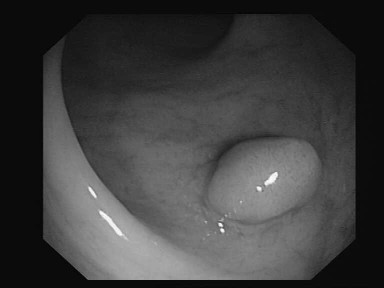
\includegraphics[width=.8\linewidth]{polyp129}
		\caption{}
		\label{fig:polyp}
	\end{subfigure}
	\begin{subfigure}{.3\textwidth}
		\centering
		
\includegraphics[width=.8\linewidth]{segm129}
		\caption{}
		\label{fig:segm}
	\end{subfigure}
	\begin{subfigure}{.3\textwidth}
		\centering
		% TODO Create graphic
		
\includegraphics[width=.8\linewidth]{segm129}
		\caption{}
		\label{fig:highlight}
	\end{subfigure}
	\caption{Kolorektalpolyp, dessen Segmentierung und Hervorhebung im Bild~\cite{Vazquez.2017}}
	\label{fig:polypseg}
\end{figure}

In der vorliegenden Masterarbeit wird zur Lösung dieses Lokalisierungsproblems ein Deep-Learning-Ansatz verwendet, der bisher noch nicht bei der Lokalisierung von Polypen eingesetzt wurde.
Dieser Ansatz, die \glspl{can} \cite{Isola.2017}, basiert auf den \glspl{gan} \cite{Goodfellow.2014}.

Dieses Kapitel erläutert die Problemstellung und stellt den Stand der Technik vor.
In den anschließenden Kapiteln erfolgt eine methodische Aufschlüsselung des Vorgehens in dieser Arbeit, die Umsetzung dieser Methodik, deren Ergebnisse und eine Analyse dieser Ergebnisse.



\section{Medizinischer Hintergrund}

\emph{Polypen} beginnen generell als leichte Erhebungen in der Schleimhaut, die in das Lumen des umgebenden Organs hineinragen~\cite{Kumar.2005}.
Anfangs wachsen sie \emph{sessil} ("stiellos") und sind nur als breite Kuppeln sichtbar, können aber im Lauf der Zeit einen Stiel entwickeln, sodass \emph{gestielte} Polypen in etwa pilzförmig aussehen.

Polypen lassen sich einteilen in \emph{neoplastisch} und \emph{nicht-neoplastisch}~\cite{Kumar.2005}.
Die häufigste neoplastische Polypenform ist das \emph{Adenom}, das sich im Laufe der Zeit zu Krebs entwickeln kann.
Alle anderen Polypenarten hingegen entwickeln sich fast ausschließlich gutartig.
Das Aussehen eines Polyps reicht in der Regel nicht aus zur Beurteilung der Malignität; dies ist bisher fast ausschließlich durch eine histologische Untersuchung des Polypengewebes möglich.
Allerdings steigt mit zunehmender Größe eines Polypen die Wahrscheinlichkeit, dass es sich um ein Karzinom handelt.

Karzinome, die sich aus Adenomen entwickeln, sogenannte \emph{Adenokarzinome}, sind die häufigste Form von bösartigen Tumoren im \gls{gi}~\cite{Kumar.2005}.
Im Kolorektalbereich, der vom allerletzten Abschnitt des Dünndarms bis zum Rektum reicht, tritt die stark überwiegende Mehrheit aller malignen Polypen im \gls{gi} auf.
Im Dünndarm hingegen treten sowohl benigne als auch maligne Polypen sehr selten auf; die Auftrittswahrscheinlichkeit sinkt weiter, je höher man im \gls{gi} aufsteigt.
In dieser Arbeit wird deshalb ausschließlich die Segmentierung von \emph{Kolorektalpolypen} betrachtet.

Zur Untersuchung des Kolorektalbereichs wird üblicherweise eine Koloskopie durchgeführt, bei der mittels eines rektal eingeführten Endoskops die gesamte Region inspiziert werden kann.
Analog dazu werden bei einer Spiegelung des Dünndarms meist oral eingeführte Endoskopkapseln eingesetzt, was als \gls{wce} bezeichnet wird.
Im Kontext dieser Arbeit wird nur auf Bildmaterial eingegangen, das durch Endoskopie im Bereich des sichtbaren Lichts produziert wurde.
Andere Modalitäten wie bspw. Narrow Band Imaging, bei dem zur besseren Hervorhebung bestimmter Gewebsarten nur bestimmte schmale Frequenzbänder des sichtbaren Lichts zum Einsatz kommen, werden hier nicht betrachtet.



\section{Problemstellung}

Um eine Hervorhebung von Polypen im koloskopischen Bild während einer Darmspiegelung zu ermöglichen, ist ein automatisiertes Auffinden von Polypen notwendig.
Diese Lokalisierung kann unterschiedlich genau sein, vom einzelnen Bildpunkt über Bounding Boxes bis hin zu ellipsenförmigen Bereichen.
Wenn ein Algorithmus in der Lage ist, die Fläche des Polypen \emph{pixelgenau} im Bild zu finden, wird in dieser Arbeit von einer \emph{Segmentierung} gesprochen als der genauesten Form der Lokalisierung.
In allen anderen Fällen wird nur von einer \emph{Lokalisierung} gesprochen.

Diese Arbeit befasst sich mit dem Einsatz einer bestimmten Deep-Learning-Architektur, um Polypen in koloskopischen Bildern zu segmentieren.
Dabei soll sowohl die Qualität der Segmentierung als auch Verbesserungen zur Stabilisierung des Trainings evaluiert werden.
In den folgenden Abschnitten werden alternative, bereits bestehende Ansätze zur Polypen-Lokalisierung und -Segmentierung vorgestellt und erläutert.
Diese werden hier aufgeteilt in solche Ansätze, bei denen die relevanten Bildmerkmale vom menschlichen Experten festgelegt werden, und solche, bei denen Features vollständig gelernt werden.

In Echtzeitszenarien kann es durchaus sinnvoll sein, zuerst einen leichtgewichtigeren Algorithmus binär detektieren zu lassen, ob ein Polyp im Bild vorhanden ist, und anschließend diese \emph{Präsenz-Detektion} durch eine Lokalisierung zu erweitern.
Im Rahmen dieser Arbeit werden Methoden zur reinen Detektion der Präsenz von Polypen allerdings nicht genauer betrachtet.

Ebenso ist die Beurteilung der Bösartigkeit des Gewebes anhand der Bildinformation, eine sogenannte "optische Biopsie", zwar ein interessantes Forschungsproblem~\cite{Roy.2011}, aber diese Arbeit hat keine derartige Klassifikation zum Ziel.
%TODO optical biopsy als Ausblick am Schluss



\section{Feature Selection}

Algorithmen, die Bilder verarbeiten, haben es in aller Regel mit sehr hochdimensionalen Daten zu tun.
Aus diesen Eingabedaten wird versucht, gehaltvolle Ausgaben zu erzeugen wie bspw. Aussagen über die Präsenz gewisser Objekte, menschliche Emotionen oder die Position bestimmter Objekte.
Um aus diesen hochdimensionalen Inputs Ausgaben mit deutlich geringerer Dimensionalität zu erzeugen, ist es notwendig, die Dimensionalität des Inputs zu reduzieren, indem man Merkmale verwirft, die für die Ausgabe nicht relevant sind.

Woher weiß der Algorithmus, welche Merkmale relevant sind?
Entweder man instruiert ihn explizit, indem man Expertenwissen fest in den Algorithmus einkodiert, oder man lässt es ihn selbstständig herausfinden.
Die erste Variante produziert zumeist Algorithmen, die sehr auf Problem und Domäne zugeschnitten und nur schwer übertragbar sind; allerdings kann man die Kriterien, anhand derer sie eine Ausgabe erzeugen, von außen nachvollziehen.
Die zweite Variante hingegen erzeugt Algorithmen, die große Mengen an Trainingsdaten benötigen, dafür aber tendentiell viel flexibler und einfacher auf andere Domänen übertragbar sind.

In diesem Abschnitt werden Ansätze zur Lokalisierung und Segmentierung von Polypen vorgestellt, die zur ersten Kategorie gehören; im darauffolgenden Abschnitt folgen Ansätze der zweiten Kategorie.



\subsection{Lokalisierung}

In \cite{Prasath.2016} reviewt \citeauthor{Prasath.2016} verschiedene Ansätze zur Detektion, Lokalisierung und Segmentierung von Polypen in \gls{wce}-Videos.
Auch wenn die Gegebenheiten der Bildgebung bei der Kapselendoskopie sich von denen der Koloskopie unterscheiden, arbeiten doch beide im Spektrum des sichtbaren Lichts, weshalb ein Vergleich von Algorithmen beider Modalitäten möglich sein sollte.

Auch wenn Ansätze zur reinen Detektion von Polypen hier nicht genauer betrachtet werden, bauen doch die Mehrheit solcher Ansätze einen Lokalisierungsschritt ein, um dann zu entscheiden, ob ein Polyp im Bild vorhanden ist~\cite{Prasath.2016}.
Bei solchen Lokalisierungen kommen meist elliptische Features, Textur, Farbe und Positionseigenschaften als Merkmale zum Einsatz.

Von den bei \cite{Prasath.2016} vorgestellten Ansätzen verlassen sich die meisten Lokalisierungen auf die Filterung von Kanten und eigens gefertige Maße für Krümmungen und Vorwölbungen im Bild.
Mithilfe dieser Features werden Lokalisierungen erzielt, die als Ausgabe einen Bildpunkt, eine Bounding Box, eine Ellipse oder eine grobe Segmentierung erzielen.
Oftmals kommen im Ablauf einzelner Algorithmen gelernte Elemente hinzu wie bspw. ein Clustering-Algorithmus zur Filterung von Lokalisierungskandidaten, aber dennoch werden die Merkmale, auf denen gelernt wird, vom Menschen ausgewählt.

Abgesehen von den in \cite{Prasath.2016} verglichenen Ansätzen geht folgende Arbeit ebenfalls dem Lokalisierungsbroblem nach:
In \cite{Li.2004} ist das Ziel eine Lokalisierung von abnormalen Regionen im koloskopischen Bild, wozu auch Regionen mit Polypen zählen.
Ausgabe ist eine binäre Segmentierung mit rechtwinkligen Grenzen, da mit Patches des Bildes gearbeitet wird, von denen jeder einzeln mittels eines Ensemble-Lerners klassifiziert wird.
Diese Patches werden auf mehreren Skalierungen erstellt, um verschiedene Abnormalitätengrößen erfassen zu können.
Features in den einzelnen Patches werden generiert durch eine Diskretisierung der Farbwerte im CIELab-Farbraum und anschließende Berechnung von Farb-Features und -Statistiken, die u.~a. von einer diskreten Wavelet-Transformation stammen.



\subsection{Segmentierung}

Bei \cite{Prasath.2016} werden auch verschiedene Segmentierungsalgorithmen für Kolorektalpolypen verglichen.
Diese basieren alle auf Varianten von \emph{Active Contours}~\cite{Kass.1988}, bei denen ein verformbares, a priori festgelegtes Linienmodell durch Energieminimierung auf ein Bild eingepasst wird.
\citeauthor{Sasmal.2018} nutzen ebenfalls Active Contours und initialisieren die Segmentierung mit kreisförmigen Löchern auf die gesamte Bildfläche~\cite{Sasmal.2018}.

\citeauthor{Ionescu.2013} halten die gekrümmte Form der Polypen für am meisten aussagekräftig und entwickeln eine eigene Methode zur Verstärkung der Polypenkanten im Bild~\cite{Ionescu.2013}.
\citeauthor{Vieira.2012} segmentieren abnormales Gewebe von normalem und nutzen dafür ein Gaussian Mixture Model basierend auf den Vektoren im HSV- und RGB-Farbraum~\cite{Vieira.2012}.




\section{Feature Learning}

Kolorektalpolypen zu lokalisieren ist komplex, denn Form, Textur und Farbe unterscheiden sich teilweise drastisch zwischen Polypen, oftmals sogar beim selben Patienten~\cite{Prasath.2016}.
Viele der vorgestellten Lokalisierungsverfahren nutzen Kombinationen dieser Features, aber die Segmentierungsverfahren verlassen sich alle ausschließlich auf die Form als entscheidendes Merkmal (bis auf einen rein farbbasierten Ansatz).
Aufgrund der hohen Varianz an Polypenaussehen kann es nicht ausreichen, sich nur auf eines dieser Merkmale zu verlassen~\cite{Prasath.2016}.

Algorithmen, die selbst explorativ herausfinden, welche Features relevant sind, lernen auf den originalen Rohdaten und können somit jegliche Kombination aus Merkmalen zur Lösung des Problems nutzen.
Die Ansätze in diesem Abschnitt basieren alle auf Feature Learning.
\emph{Deep Learning} ist hierbei das Konzept, das Feature Learning bisher am erfolgreichsten ganzheitlich inkorporiert.
Anders als bestimmte Clusteringverfahren oder die \gls{pca}~\cite{Hotelling.1933}, die sich darauf beschränken aussagekräftige Merkmale zu finden, ermöglicht Deep Learning nicht nur das Erlernen von Features, sondern auch das Lernen von Mappings von Merkmalswerten zu gewünschten Ausgaben.

Deep Learning bezeichnet eine Klasse von Algorithmen, bei denen künstliche \glspl{nn} zum Einsatz kommen, die mehr als eine verborgene Schicht besitzen~\cite{Goodfellow.2016}.
Viele lernende Algorithmen kommen nur mit Problemen in niedrigdimensionalen Räumen zurecht, weil sie theoretisch für jeden möglichen Punkt im Merkmalsraum Trainingsbeispiele benötigen.
Abgesehen von diesem "Fluch der Dimensionalität"~\cite{Bellman.2010} stützen sich viele Lernalgorithmen auf die Annahme, dass die zu lernende Funktion in kleinen, lokalen Bereichen ungefähr konstant verläuft, was aber nicht immer der Fall sein muss.
Beiden Problemen kann Deep Learning entgegentreten durch das Lernen von niedrigdimensionalen, nicht-lokalen Mannigfaltigkeiten im Merkmalsraum~\cite{Bengio.2005} und durch die Annahme, dass die Trainingsdaten durch mehrere zugrundeliegende Faktoren, möglicherweise auf mehreren Abstraktionsebenen, verursacht wurden~\cite{Goodfellow.2016}.
Gerade letztere Hypothese bietet sich sehr gut für das hier vorliegende Segmentierungsproblem an, da das Zusammenwirken verschiedener Faktoren eine Grundannahme ist.

Generell bieten Features lernende Algorithmen einen weiteren Vorteil gegenüber solchen mit selektierten Features:
Es ist kaum Vorverarbeitung notwendig, da der Algorithmus selbstständig lernt, welche Informationen des Originalinputs nicht relevant sind.
Aufwendiges Entfernen von Glanzlichtern oder das Limitieren des Gesamtbildes auf eine Interessenregion entfällt, was gerade bei den Ansätzen im vorherigen Abschnitt sehr häufig eingebaut wird.



\subsection{Convolutional Neural Networks}

Eine Deep-Learning-Architektur, die besonders im Bereich der Bildverarbeitung sehr verbreitet ist, ist das \gls{cnn}.
In dieser Variante von tiefen \glspl{nn} wird in mindestens einer Schicht die Faltungsoperation angewandt.
Die Werte einer Kernelmatrix, die für eine Neuronenschicht in jedem Bildfenster gleich bleibt, werden vom Netz gelernt.
Da die Neuronen in \glspl{cnn} mehr Parameter untereinander teilen als Netze mit vollständig verbundenen Schichten, die einer Matrixmultiplikation entspricht, ist ihre Speicherkomplexität geringer.

Durch den Einsatz von Pooling-Schichten oder Faltungsschichten mit größeren Strides sind \glspl{cnn} außerdem in der Lage, Repräsentationen zu lernen, die gegenüber kleinen Verschiebungen im Input invariant sind.
Dies wiederum drückt eine A-Priori-Annahme in \glspl{cnn} aus, die sich für Bilder sehr gut eignet:
Geringe Translationen sollten die Semantik eines Bildes nicht verändern.

Damit \glspl{cnn} gut generalisieren, benötigen sie in der Regel sehr viele Trainingsdaten.
In vielen Fällen lässt sich ein Netz, das schon für ein bestimmtes Problem trainiert wurde, als Ausgangspunkt für ein neues Netz nehmen, welches das bereits trainierte Netz nur noch leicht anpassend nachtrainiert auf das neue Zielproblem.
Dieses \emph{Transfer Learning} kann den Bedarf an Trainingsdaten deutlich verringern.
Gerade im Bereich der Objekterkennung haben sich viele Deep-Learning-Architekturen etabliert, die auf großen, gelabelten Bilddatenbanken wie ImageNet~\cite{Deng.2009} trainiert wurden und deren erste Schichten gerne als Startpunkt für neue Objekterkennungsnetze in speziellen Domänen genutzt werden (s. z.~B.~\cite{Simonyan.2014}).



\subsection{Lokalisierung}





\subsection{Segmentierung}





\subsection{Generative Netze}





\section{Fazit}



\chapter{Material und Methoden}

Dieses Kapitel stellt die Deep-Learning-Architektur und das Dataset genauer vor, mit dem sich diese Thesis beschäftigt.
Grundlage der \glspl{can} sind die \glspl{gan}, weshalb diese zuerst betrachtet werden.
Anschließend erfolgt eine Erläuterung zur Architektur der \glspl{can} und welche Besonderheiten in Bezug auf die Segmentierung auftreten.
Zum Schluss wird das Datenmaterial vorgestellt, das in dieser Arbeit zum Einsatz kommt.



\section{Generative Adversarial Networks}

Maschinelles Lernen hat eine Klasse Algorithmen hervorgebracht, die sehr viele gelabelte Daten benötigen.
Um die Menge an benötigten Daten zu verringern, wird im Deep-Learning-Bereich an Ansätzen geforscht, die neue Trainingssamples generieren, fehlende Werte ausfüllen oder durch unüberwachtes Lernen oder Transfer Learning zu einer Verbesserung beitragen können~\cite{Goodfellow.2016}.
Viele dieser Entwicklungen basieren auf Modellen, die Wahrscheinlichkeitsverteilungen über die Trainingsdaten abschätzen, und solche Abschätzungen sind nur durchführbar, wenn man Inferenz approximiert.

Eine solche approximierte Inferenz bedingt eine Normalisierung über eine Konstante, deren Berechnung wiederum nur durch Approximation durchführbar wird.
Viele dieser Approximationen werden wegen der Abhängigkeit von allen Modellparametern mit wachsender Dimensionalität exponentiell schwieriger zu berechnen.
Häufig werden auf Markov-Ketten basierende Monte-Carlo-Methoden~\cite{Koller.2009} zur Berechnung der Normalisierungskonstante genutzt, aber diese funktionieren meist nur bei Konstellationen mit wenigen, nicht klar separierten Moden der Wahrscheinlichkeitsverteilung~\cite{Goodfellow.2016}.

Die \glspl{gan} von \citeauthor{Goodfellow.2014}~\cite{Goodfellow.2014} umgehen diese Herausforderungen durch die Gestaltung ihrer Architektur.
Ihr spieltheoretisch motivierter Ansatz, in dem zwei Netze gegeneinander arbeiten, ist mit Backpropagation trainierbar und benötigt somit weder approximierte Inferenz noch unkalkulierbare Normalisierungskonstanten.
Das Ziel ist es, möglichst realistisch wirkende Samples zu generieren.
\emph{Realistisch} bedeutet in diesem Kontext, dass ein erzeugtes Sample $ \mathbf{x} $ den Trainingsdaten sehr ähnlich, aber nicht identisch sein soll.

Das erste Netz, der \emph{Generator} $ G $, lernt eine Wahrscheinlichkeitsverteilung $ p_{\textup{data}}(\mathbf{x}) $ über die Trainingsdaten.
Aus einem zufällig initialisierten Vektor $ \mathbf{z} $ erzeugt er dann neue Samples.
Parallel dazu lernt das andere Netz, der \emph{Diskriminator} $ D $, immer besser zu beurteilen, ob ein Sample $ \mathbf{x} $ realistisch ist oder \emph{gefälscht}, also ob es aus den Trainingsdaten stammt oder vom Generator erzeugt wurde.

Der Generator versucht nun die Wahrscheinlichkeit zu maximieren, dass der Diskriminator einen Fehler macht und ein Sample falsch beurteilt~\cite{Goodfellow.2014}.
Als Zielfunktion ergibt sich

\begin{equation}\label{eq:gan}
\mathcal{L}(D, G) = \mathbb{E}_{\mathbf{x} \sim p_{\textup{data}}(\mathbf{x})} [\log D(\mathbf{x})] + \mathbb{E}_{\mathbf{z} \sim p_{\mathbf{z}}(\mathbf{z})} [\log(1 - D(G(\mathbf{z})))].
\end{equation}

Die eigentliche Verlustfunktion ist dann

\begin{equation}\label{eq:ganrisk}
R = \textup{arg}\min_G \max_D \mathcal{L}(D, G).
\end{equation}

Um Overfitting in $ D $ zu vermeiden, werden beide Netze von Grund auf trainiert, wobei bei jedem Trainingsschritt alterniert wird zwischen einem Update in $ D $ und einem Update in $ G $.
Es lässt sich zeigen, dass $ G $ auf diese Weise implizit eine Wahrscheinlichkeitsverteilung lernt, die den Trainingsdaten entspricht~\cite{Goodfellow.2014}.
Da $ D $ einen Skalar zwischen 0 und 1 ausgibt als Bewertung für die Realitätsnähe eines Samples, wird das Training als abgeschlossen betrachtet, wenn $ D $ für Samples aus den Trainingsdaten und generierte Samples den gleichen Wert ausgibt, nämlich $ \frac{1}{2} $.
In diesem Zielzustand kann der Diskriminator nicht mehr zwischen realen und gefälschten Samples unterscheiden; er kann dann verworfen werden.

Die visuelle Qualität der Erzeugnisse der originalen \glspl{gan} wurde in darauffolgenden Arbeiten deutlich verbessert.
Besonders die LAPGANs und \glspl{dcgan} haben sich hierbei hervorgetan.



\subsection{LAPGANs}

Die LAPGANs von \citeauthor{Denton.2015}~\cite{Denton.2015} basieren auf einer Laplace'schen Pyramide, bei der auf jeder Ebene ein gesondertes \gls{gan} eine Bildschärfung lernt.
Am Anfang erzeugt das erste \gls{gan} $ G_1 $ ein Sample mit sehr niedriger Auflösung, welches anschließend hochskaliert wird.
Das \gls{gan} der zweiten Ebene $ G_2 $ nimmt dann dieses hochskalierte, unscharfe Bild, und generiert dazu ein Restbild.
Dieses wird zum hochskalierten Bild addiert, das Ergebnis wird wieder hochskaliert und an die nächste Ebene weitergereicht, wo die nächste Schärfung stattfinden kann.
Der Prozess ist in \autoref{fig:lapgansampling} dargestellt.

\begin{figure}
	\centering
	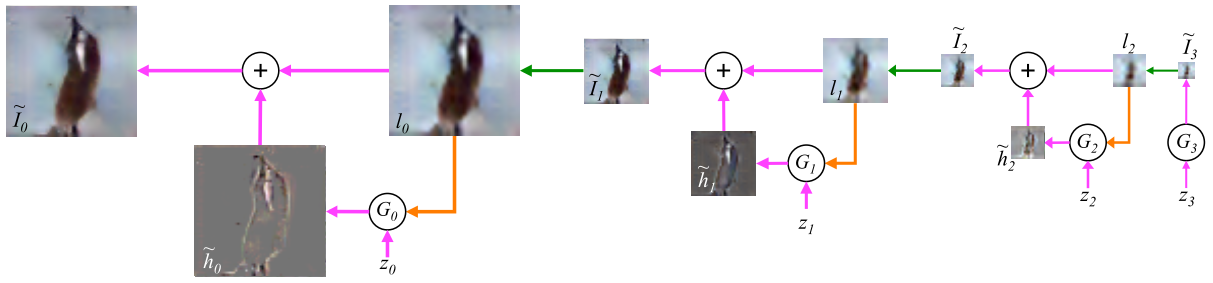
\includegraphics[width=0.9\linewidth]{img/lapgan_sampling}
	\caption{Sampling-Prozedur in LAPGANs (von rechts nach links)~\cite{Denton.2015}.}
	\label{fig:lapgansampling}
\end{figure}

Bis auf das erste \gls{gan} wird in diesem Fall auf jeder Ebene bereits eine konditionierte Variante der originalen \glspl{gan} verwendet.
Diese Modellvariante wurde schon bei \citeauthor{Goodfellow.2014}~\cite{Goodfellow.2014} vorgeschlagen und auch vor den LAPGANs bereits umgesetzt~\cite{Gauthier.2014,Mirza.2014}.
Im Kontext der konditionierten \glspl{gan} kommt eine konditionierende Variable $ \mathbf{y} $ hinzu, die sowohl an $ G $ als auch an $ D $ im Training und zur Inferenzzeit übergeben wird.
Dies erweitert die Zielfunktion von \autoref{eq:gan} zu

\begin{equation}\label{eq:canloss}
\begin{split}
\mathcal{L}_c(D, G) = & \ \mathbb{E}_{\mathbf{x}, \mathbf{y} \sim p_{\textup{data}}(\mathbf{x}, \mathbf{y})} [\log D(\mathbf{x}, \mathbf{y})] \\
+ & \ \mathbb{E}_{\mathbf{z} \sim p_{\mathbf{z}}(\mathbf{z}), \mathbf{x} \sim p_{\textup{data}}(\mathbf{x})} [\log(1 - D(\mathbf{x}, G(\mathbf{x}, \mathbf{z})))].
\end{split}
\end{equation}



\subsection{Deep Convolutional GANs}

Die \glspl{dcgan} von \citeauthor{Radford.2016}~\cite{Radford.2016} sind eine Weiterentwicklung der \glspl{gan}, deren Samples im Vergleich zu den LAPGANs weniger verrauscht sind.
Sie modifizieren die originalen \glspl{gan}, indem sie ähnlich den \glspl{fcn} nur noch Faltungsschichten statt Pooling- und vollständig verbundenen Schichten.
Außerdem nutzen sie in allen Schichten Batch-Normalisierung, was Mittelwert und Standardabweichung jedes Units einer Schicht auf respektive 0 und $ \pm 1 $ normiert.
Ebenso kommt als Aktivierungsfunktion im Generator nur noch das \gls{relu}~\cite{Nair.2010} und im Diskriminator das Leaky ReLU zum Einsatz; in der Ausgabeschicht des Generators erweist sich die Aktivierungsfunktion mit $ \tanh $ als erfolgreicher im Vergleich zu maxout bei den originalen \glspl{gan}.

Durch verschiedene Experimente können die Autoren zeigen, dass der latente Vektorraum, den das Modell lernt, tatsächlich glatte Übergänge hat, und dass die gelernten Filter zu häufig auftretenden Objekten korrespondieren.
Ebenso beobachten sie, dass das Unterdrücken von bestimmten Filtern dem Auslassen oder Transformieren bestimmter Objekte im generierten Sample entspricht, und dass simple Vektorarithmetik im latenten Vektorraum plausible Ergebnisse erzielt (s.~\autoref{fig:dcganarithmetic}).
All dies spricht dafür, dass diese Architektur nicht nur visuell ansprechende Ergebnisse erzielen kann, sondern auch eine stabile Repräsentation gelernt hat anstatt auswendig zu lernen und damit Overfitting zum Opfer zu fallen.

\begin{figure}
	\centering
	
\includegraphics[width=0.9\linewidth]{img/dcgan_arithmetic}
	\caption{Beispiel für Vektorarithmetik in \glspl{dcgan}~\cite{Radford.2016}.}
	\label{fig:dcganarithmetic}
\end{figure}



\section{Conditional Adversarial Networks}

Die \glspl{can} von \citeauthor{Isola.2017}~\cite{Isola.2017} bestehen aus einem Generator und einem Diskriminator, die beide auf \glspl{dcgan} basieren.
Ihr Ansatz ist mit dem Zweck gestaltet, eine generische Architektur für Probleme bereitzustellen, bei denen eine Repräsentation eines Bildes auf eine andere Repräsentation eines Bildes abgebildet wird; die Autoren sprechen in diesem Zusammenhang von "Bild-zu-Bild-Übersetzung".

Im Gegensatz zu anderen Arbeiten, die konditionierte \glspl{gan} für spezielle Bild-zu-Bild-Probleme verwenden, ist in ihrer Architektur theoretisch \emph{nichts} anwendungsspezifisch angepasst.
Stattdessen ermöglicht es das GAN-Framework, dass die konkrete Verlustfunktion vollständig aus den Trainingsdaten gelernt wird, ohne dass diese problemspezifisch von Hand definiert werden muss.



\subsection{Generator}

Der Generator der \glspl{can} basiert auf dem \gls{dcgan}, muss aber in der konditionierten Variante erweitert werden, damit das Inputbild $ \mathbf{y} $ bei der Eingabe in den Generator herunterskaliert und dadurch enkodiert werden kann.
Man könnte dafür den Aufbau eines Encoder-Decoders wählen; tatsächlich orientiert sich der Generator konkret an der Struktur des U-Net~\cite{Ronneberger.2015}:
Diese Netzvariante ähnelt den \glspl{fcn}~\cite{Long.2015}, die bereits Skip Connections einbauen, damit trotz der Herunterskalierung Information aus den ursprünglichen Skalenstufen in die späteren Schichten des Netzes fließen kann.
Beim U-Net werden allerdings im Gegensatz zum FCN-8s nicht nur die niedrigsten drei Skalierungsstufen verbunden, sondern jede Schicht $ i $ wird mit der "gegenüberliegenden" Schicht $ n-i $ verbunden (s.~\autoref{fig:unetarchitecture}).
Zusätzlich entsprechen diese Skip Connections nicht der elementweisen Aufsummierung, sondern aus einem Anhängen der Kanäle von Schicht $ i $ an die Kanäle der späteren Schicht $ n-i $.

\begin{figure}
	\centering
	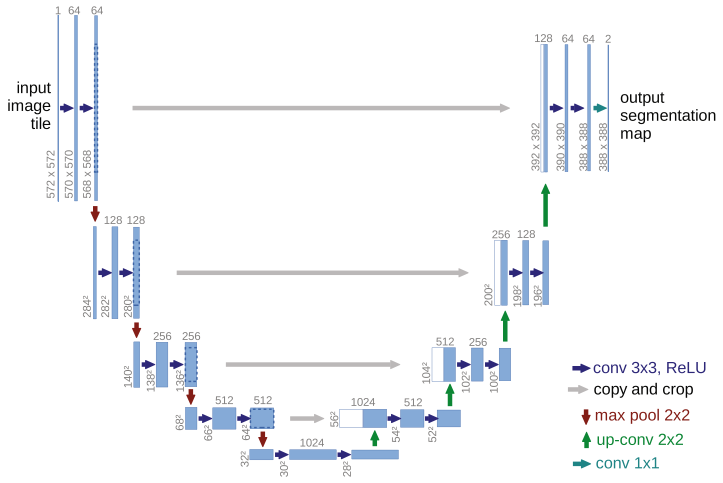
\includegraphics[width=0.7\linewidth]{img/unet_architecture}
	\caption{Architektur des U-Net~\cite{Ronneberger.2015}.}
	\label{fig:unetarchitecture}
\end{figure}



\subsection{Diskriminator}

Die Formulierung des Diskriminators in einem \gls{gan} entscheidet darüber, wie erfolgreich der Generator lernen kann, weil der Diskriminator ihm aufzeigt, welche Outputs realistisch wirken.
Damit der Diskriminator entscheiden kann, wie realistisch das Bild $ G(\mathbf{x}, \mathbf{y}) $ aussieht in Abhängigkeit vom Inputbild $ \mathbf{y} $, muss er ein Maß haben, um Bilder miteinander vergleichen zu können.
\citeauthor{Isola.2017} gestalten hier sowohl die Verlustfunktion als auch den Diskriminator ausgehend von der Hypothese, dass die niedrigen Frequenzen im Bild von herkömmlichen Distanzfunktionen sehr gut modelliert werden, aber die hohen Bildfrequenzen durch gelernte Funktionen abgedeckt werden müssen.

Verbreitete Maße zum Vergleich von Bildern sind die L1-Distanz mit $ \sum_i | \mathbf{x}_i - \mathbf{y}_i | $ und die L2-Distanz mit $ \sum_i (\mathbf{x}_i - \mathbf{y}_i)^2 $.
Solche pixelweisen Differenzen nehmen den Eingaberaum als unstrukturiert wahr.
Nutzt man ein solches Distanzmaß als Verlustfunktion in einem \gls{gan}, das Bilder generiert, kommen dabei meist nur unscharfe und graue Bilder heraus.
Scheinbar produziert der Einsatz dieser Maße eine unscharfe Ausgabe, wenn sie eine Bildkante nicht genau lokalisieren können, bzw. eine gemittelte graue Farbe, wenn sie eine auffällige Farbe nicht genau lokalisieren können~\cite{Isola.2017}.
Allerdings sind diese Maße in der Lage die groben Strukturen, also die tiefen Frequenzen im Bild, treffend abzubilden.
Deshalb kommt zur Einhaltung der Korrektheit in den tiefen Frequenzen die L1-Distanz in der Verlustfunktion zum Einsatz.

Der Diskriminator hingegen wird als \emph{PatchGAN} aufgebaut, der die feinen Strukturen und damit die hohen Frequenzen im Bild auf Realitätsnähe überprüfen kann.
(Der Name des Diskriminators ist irreführend gewählt, da es sich bei dem Diskriminator nicht um ein \gls{gan} handelt -- besser wäre vermutlich so etwas wie \emph{Patch-Diskriminator}.)
Dieser Diskriminator ist als Netzstruktur aufgebaut, die einen Filter mit fester Größe faltend auf dem gesamten Bild einsetzt.
Eine zu kleine Größe des Filters erzeugt Bilder, die kachelartige Artefakte aufweisen; ein Filter mit der vollen Bildgröße skaliert nicht gut für Bilder mit beliebiger Größe und liefert nicht so gute Ergebnisse wie ein Filter mit 70$\times$70 Pixeln.
Die Ausgabe des Diskriminators sind die Aktivierungen seiner letzten Schicht, was einer 30$\times$30-Matrix entspricht, wobei jedes Element dieser Matrix der Glaubwürdigkeit eines 70$\times$70-Ausschnitt des Bildes entspricht.

Diese Formulierung des Diskriminators drückt prinzipiell die gleiche Annahme wie die eines \gls{mrf} aus:
Ein Pixel ist nur von den Pixeln unabhängig, die von ihm durch einen gewissen Abstand getrennt sind.



\subsection{Verlustfunktion}

Die Verlustfunktion für konditionierte \glspl{gan} (s.~\autoref{eq:ganrisk}) wird bei den \glspl{can} von \citeauthor{Isola.2017} in zwei Punkten modifiziert:
Zum einen wird die im vorigen Abschnitt erwähnte L1-Distanz hinzugefügt, zum anderen wird der Rauschvektor ausgelassen.
Um die niedrigen Bildfrequenzen korrekt im \gls{can} zu modellieren, wird ein gewichteter L1-Term in der Verlustfunktion hinzugefügt:

\begin{equation}
R^* = \textup{arg}\min_G \max_D \mathcal{L}_c(D, G) + \lambda \mathcal{L}_{L1}(G)
\end{equation}

Die hohen Bildfrequenzen können dann durch die beiden Terme des Diskriminators im ersten Summanden abgedeckt werden (s. \autoref{eq:canloss}), die niedrigen Frequenzen werden durch den zweiten Summanden modelliert.
Die besten Ergebnisse über alle Bild-zu-Bild-Übersetzungsaufgaben wurde erzielt für $ \lambda = 100 $.

In der Zielfunktion der \glspl{gan} spielt der Rausch-Vektor $ \mathbf{z} $ als Startpunkt für $ G $ eine wichtige Rolle, damit der Generator überhaupt eine Ausgabe erzeugen kann.
Da der Generator allerdings bei den \glspl{can} bereits einen Input erhält, ist dieser nicht mehr notwendig und es ergibt sich folgende Formulierung der Zielfunktion:

\begin{equation}\label{eq:canlosswonoise}
\begin{split}
\mathcal{L}_c(D, G) = & \ \mathbb{E}_{\mathbf{x}, \mathbf{y} \sim p_{\textup{data}}(\mathbf{x}, \mathbf{y})} [\log D(\mathbf{x}, \mathbf{y})] \\
+ & \ \mathbb{E}_{\mathbf{x} \sim p_{\textup{data}}(\mathbf{x})} [\log(1 - D(\mathbf{x}, G(\mathbf{x})))].
\end{split}
\end{equation}

Rauschen wird zur besseren Stabilisierung des Trainings dennoch in Form von Dropout eingesetzt.

Die Autoren stellen zu Beginn ihres Ansatzes die Behauptung auf, dass die Verlustfunktion vollständig vom Netz gelernt wird und nicht für jedes Problem neu angepasst werden muss.
Dies ist nur insofern richtig, als dass die Probleme als Bild-zu-Bild-Übersetzung formuliert werden können.
Erstaunlich viele Aufgaben lassen sich als diese Klasse von Problemen betrachten, darunter Bildrekonstruktion aus Kantenbildern, Style-Transfer und Kolorierung von Graustufenbildern\footnote{Weitere Beispiele s. \url{https://phillipi.github.io/pix2pix/}}.
Auch semantische Segmentierung kann als ein solches Problem verstanden werden.



\subsection{Segmentierung}

Segmentierung wird in der Literatur klassischerweise definiert als

\begin{quote}Aufteilung des Bildes in mehrere verschiedene Regionen, wobei jede dieser Regionen gewisse Informationen oder Eigenschaften besitzt.~\cite[S.~29]{Ens.2011}\end{quote}

Im Fall der \emph{semantischen Segmentierung} sind diese Regionen \emph{Segmente} des Bildes, die Instanzen von bestimmten Objekten oder Gruppen solcher Objekte enthalten.
Bei einer Segmentierung mehrerer Klassen wird meist jedes Segment mit einer eigenen Farbe pixelgenau repräsentiert (s.~\autoref{fig:segnet_multiclassseg}), bei \emph{binären} Segmentierung mit nur einer zu segmentierenden Objektklasse wird meist ein Binärbild ausgegeben, wobei die Segmente weiß und der Hintergrund schwarz ist (s.~\autoref{fig:unet_binaryseg}).

\begin{figure}
	\centering
	\begin{subfigure}{.45\textwidth}
		\centering
		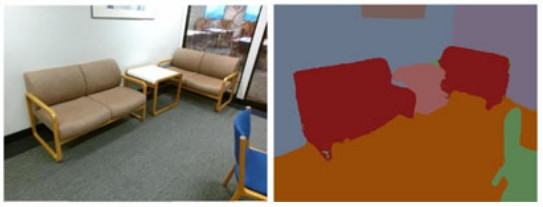
\includegraphics[width=0.9\linewidth]{img/segnet_multiclassseg}
		\caption{}
		\label{fig:segnet_multiclassseg}
	\end{subfigure}
	\begin{subfigure}{.45\textwidth}
		\centering
		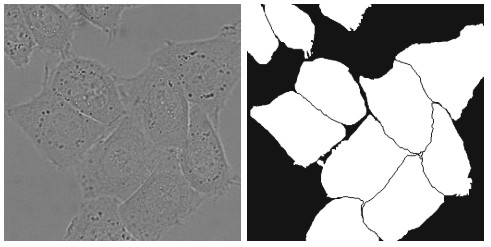
\includegraphics[width=0.9\linewidth]{img/unet_binaryseg}
		\caption{}
		\label{fig:unet_binaryseg}
	\end{subfigure}
	\caption{Beispiel von (a) Multiklassen-Segmentierung~\cite{Badrinarayanan.2017} und (b) binärer Segmentierung~\cite{Ronneberger.2015}.}
\end{figure}

\citeauthor{Isola.2017} überprüfen auch den Anwendungsfall einer semantischen Segmentierung mit einem Dataset von segmentierten Straßenszenen, wobei mehrere Objektklassen auftreten.
Die Kombination aus \gls{can} und L1-Distanz schneidet dabei schlechter ab als eine Verwendung von nur L1 als Verlustfunktion; letzteres liefert die besten Ergebnisse.
Scheinbar tendiert das \gls{can} dazu, übereifrig viele kleine Objekte zu segmentieren, die im Originalbild gar nicht vorkommen (s.~\autoref{fig:canseg}).

\begin{figure}
	\centering
	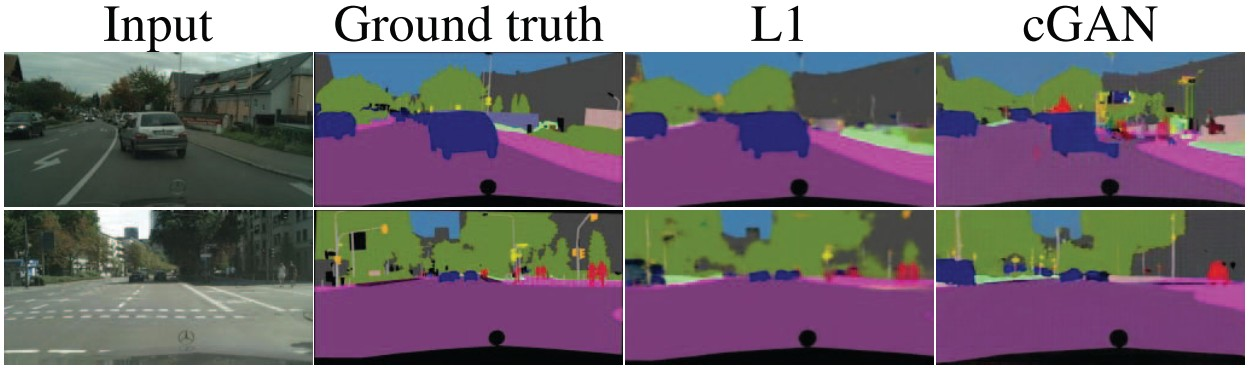
\includegraphics[width=0.9\linewidth]{img/can_seg}
	\caption{Ergebnisse von Multi-Klassen-Segmentierung bei \glspl{can}~\cite{Isola.2017}.}
	\label{fig:canseg}
\end{figure}

Zusätzlich produziert das \gls{can} keine vollständig diskreten Ergebnisse, bei denen die Segmentgrenzen klar sind, sondern tendenziell können auch Farbverläufe auftreten.
Allerdings wurde das \gls{can} noch nicht für eine binäre Segmentierung verwendet, was eben in dieser Arbeit getan wird.



\section{Dataset}

In dieser Arbeit wird eine binäre semantische Segmentierung von Kolorektalpolypen mittels eines \gls{can} durchgeführt.
Für das Training des \gls{can} ist ein Dataset notwendig, das in diesem Fall im Rahmen der \gls{giana} Challenge 2018\footnote{\url{https://giana.grand-challenge.org/}} zur Verfügung gestellt wurde.
Diese Challenge ist eine Sub-Challenge der Endoscopic Vision Challenge, die wiederum Teil der MICCAI-Konferenz ist.
Die Endoscopic Vision Challenge findet seit 2015 statt\footnote{\url{https://endovis.grand-challenge.org/}} und hat es sich zum Ziel gesetzt, den aktuellen Stand der Technik im Bereich der medizinischen Bildverarbeitung mithilfe von öffentlich ausgerufenen Sub-Challenges und Datasets zu evaluieren.

Das Dataset der \gls{giana} Sub-Challenge ist eine Kombination verschiedener Datasets, die auch schon in vorherigen Challenges öffentlich gemacht wurden~\cite{Bernal.2012,Bernal.2015,Vazquez.2017}.
Eine Übersicht der Datasets ist in \autoref{tab:datasets} abgebildet.

\begin{table}
	\centering
	\caption{Details zu den Datasets}
	\label{tab:datasets}
	\begin{tabular}{cccccc} 
		\toprule
		Database     & \begin{tabular}[c]{@{}c@{}}Anzahl\\Patienten \end{tabular} & \begin{tabular}[c]{@{}c@{}}Anzahl\\Sequenzen \end{tabular} & \begin{tabular}[c]{@{}c@{}}Anzahl\\Frames \end{tabular} & Auflösung         & \begin{tabular}[c]{@{}c@{}}Zugehörigkeit\\Split \end{tabular}  \\ 
		\midrule
		CVC-ColonDB  & 13                                                         & 13                                                             & 300                                                     & 500$\times$574    & Training                                                       \\
		CVC-PolypHD  & (*)                                                          & (*)                                                              & 56                                                      & 1920$\times$1080  & Training                                                       \\
		CVC-ClinicDB & 23                                                         & 31                                                             & 612                                                     & 384$\times$288    & Test                                                           \\
		\bottomrule
	\end{tabular}
	Nicht offiziell bekannte Werte sind mit (*) gekennzeichnet.
\end{table}

Jeder Datensatz besteht aus einem Koloskopiebild, das unter Weißlicht-Endoskopie aufgenommen wurde, und einem dazugehörigen Ground-Truth-Binärbild, in dem pixelgenau annotiert ist, welcher Teil des Bildes zu einem Polypen gehört.
Ersteres wird im folgenden als \emph{Input}, letzteres als \emph{Target} bezeichnet.
Weiß steht im Target für die Polypen-Klasse, Schwarz für den Hintergrund.
In \autoref{fig:polyp} und \autoref{fig:segm} ist ein beispielhafter Datensatz abgebildet, bestehend aus Input und Target.

\chapter{Umsetzung}

Dieses Kapitel beschreibt die Umsetzung der gewählten Methodik mit den zur Verfügung stehenden Materialien.
Dazu wird auf das gewählte Framework, die Vorverarbeitung des Datasets und die durchgeführten Experimente eingegangen.



\section{TensorFlow}

Zur Entwicklung des \gls{can} wurde das Deep-Learning-Framework \emph{TensorFlow}~\cite{Abadi.2016} gewählt.
TensorFlow liegt ein Paradigma zugrunde, nach dem das Modell zuerst als Graph mit Entitäten und Operationen definiert und erst dann schrittweise trainiert wird.
Im Gegensatz zu imperativen Frameworks wie PyTorch ist dadurch zwar insbesondere das Debugging erschwert, aber diese gewählte Architektur sorgt dafür, dass viele Rechenoperationen im Voraus vereinfacht und teilweise auch parallelisiert werden können, sodass das Training insgesamt schneller abläuft~\cite{Goodfellow.2016}.

\citeauthor{Isola.2017} stellen den originalen Code ihrer Publikation, der in Torch geschrieben ist, online zur Verfügung\footnote{\url{https://github.com/phillipi/pix2pix}}.
Portierungen auf andere Python-basierte Frameworks wurden bereits geschrieben, darunter auch mehrere für TensorFlow.
Gewählt wurde in dieser Arbeit die TensorFlow-Portierung von Christopher Hesse\footnote{\url{https://github.com/affinelayer/pix2pix-tensorflow}}, da diese von allen am besten dokumentiert ist.

Diese Portierung konnte nur mit der TensorFlow-Version 1.5.0 nutzbar gemacht werden, da sie seit etwa 8 Monaten nicht mehr aktiv weiterentwickelt wurde.
Dadurch stehen die Kernfunktionalitäten von TensorFlow zur Verfügung, besonders praktische Weiterentwicklungen wie die Eager Execution zur unmittelbaren Evaluierung von Graph-Komponenten aber nicht.
Da kein GPU zur Verfügung stand, wurde die CPU-basierte Variante von TensorFlow genutzt.



\section{Vorverarbeitung}

Intern nimmt der Code die Bilddaten als Kombination aus Input und Target an.
Hierbei muss für jedes Input-Target-Paar ein Bild generiert werden, welches das Target rechts vom Input platziert, sodass ein zusammengesetztes Bild mit doppelter Breite entsteht.
Ein Datensatz aus CVC-300 (s.~\autoref{tab:datasets}) hat dann bspw. die Auflösung 1000$\times$574.

Im originalen Code sind außerdem nur die Dateiformate \gls{jpg} und \gls{png} erlaubt.
Das Dataset enthält allerdings eine Mischung aus \gls{bmp} und \gls{tiff} (s.~\autoref{tab:dataformats}).
TensorFlow bietet native Methoden, um mit dem BMP-Format umzugehen, also wurde der Code erweitert, sodass \gls{bmp} als Eingabeformat für Datensätze möglich wird.
Für \gls{tiff} bietet TensorFlow allerdings keine Verarbeitungsmöglichkeiten.
Da die Targets Binärbilder sind und deshalb nicht mit verlustbehafteten Kompressionsverfahren wie bei \gls{jpg} behandelt werden sollten, wurde folgendes Verfahren gewählt:
Alle Input-Bilder wurden zu \gls{bmp} konvertiert und alle Target-Bilder wurden zu \gls{png} konvertiert, sofern sie jeweils noch nicht in diesem Format vorlagen.
Die kombinierten Input-Target-Bilder wurden dann als \gls{png} produziert.

\begin{table}
	\centering
	\caption{Dateiformate der Datasets}
	\label{tab:dataformats}
	\begin{tabular}{ccc} 
		\toprule
		Sub-Dataset & Input & Target \\ 
		\midrule
		CVC-300 & \gls{bmp} & \gls{bmp} mit nur 1 Kanal \\
		CVC-612 & \gls{tiff} & \gls{tiff} \\
		CVC-HDTrain & \gls{bmp} & \gls{tiff} \\
		CVC-HDTest & \gls{bmp} & \gls{tiff} \\
		\bottomrule
	\end{tabular}
\end{table}



\subsection{Aufteilung der Splits}

Für ein Training von maschinellen Lernverfahren ist es üblich, das Dataset in mehrere Untergruppen aufzuteilen.
Meistens werden die Daten aufgeteilt in Sets für das Training, die Validierung und das Testen~\cite{Guyon.1997}.
Die Daten des Trainings-Split werden dem Netz direkt zur Verfügung gestellt, um Gradienten zu berechnen und daraus Parameter-Updates abzuleiten.
In regelmäßigen Abständen wird das Netz auf den Daten des Validierungs-Splits ausgeführt, um sicherzustellen, dass das Netz auch auf nicht gesehenen Daten gut vorhersagt und kein Overfitting stattfindet.
Am Ende des Trainings wird der Algorithmus auf dem Test-Split evaluiert, der in der Regel größer als der Validierungs-Split ist.

Das Größenverhältnis dieser Splits zueinander lässt sich zwar rechnerisch bestimmen~\cite{Guyon.1998,Guyon.1997}, allerdings sind die Verfahren ziemlich komplex.
Oftmals werden Größenverhältnisse zwischen Training- und Test-Set von 75:25 bis 90:10 vorgeschlagen.
Im Rahmen der \gls{giana} Challenge ist die Einteilung in Training- und Test-Set bereits vorgegeben.
Bezogen auf die Anzahl der \emph{Samples} macht der Test-Split beim SD-Dataset 67~\% und beim HD-Dataset 66~\% aus, was die üblichen Größenverhältnisse beinahe umkehrt.
Betrachtet man allerdings die Anzahl der Pixel, kommt zumindest beim SD-Dataset der Test-Split auf nur 44~\% des Datasets, da dessen Auflösung geringer ist.

In dieser Arbeit wurde die Aufteilung des Training-Sets in die Splits für Training und Validierung pro Dataset im Verhältnis 80:20 gewählt.
Wie später beschrieben, wird in dieser Arbeit nur das SD-Dataset verwendet.
Das gewählte Verhältnis ist ein Kompromiss zwischen den Zielen, so viel wie möglich der Trainingsdaten beim Lernen zu nutzen und gleichzeitig so viel Varianz wie möglich im Validierungsset abzubilden.
Konkret entspricht der Anteil des Validierungssets beinahe der fünffachen Menge der Sequenzen, wodurch bei zufälligem Sampling des Validierungsset optimalerweise von jeder Sequenz mindestens ein Datensatz enthalten ist.
Wünschenswert wäre eine Einteilung dieser beiden Splits nach \emph{Patienten} gewesen wie bei \citeauthor{Vazquez.2017}~\cite{Vazquez.2017}, aber die Zuordnung von Datensätzen zu Patienten ist weder öffentlich zugänglich noch direkt aus den Daten ersichtlich.



\subsection{Auflösung der Bilddaten}

Das \gls{can} kann, wie viele Deep-Learning-Architekturen, die auf Bilddaten arbeiten, nativ nur mit quadratischen Bildern umgehen, konkret mit einer Seitenlänge von 256 Pixeln.
Sowohl das Einlesen der Datensätze als auch die Ausgabe des Generators bereitet in diesem Fall Probleme, da keines der Bilder in den Datasets die passende Auflösung noch das richtige Seitenverhältnis hat.



\subsubsection{Einlesen}

Viele der Datensätze haben zwar schwarze Ränder, die keine Information enthalten, und nach deren Entfernen man ein ungefähr quadratisches Bild erhalten würde.
Allerdings sind die relevanten Bildausschnitte je nach Bildsequenz anders im Gesamtbild positioniert.
Um dieser Varianz gerecht zu werden und gleichzeitig möglichst keine Bildinformation zu verlieren, wurde die längere Bildseite als Seitenlänge des neuen quadratischen Bildes gewählt, der originale Bildinhalt horizontal und vertikal zentriert und der Rest des Bildes mit Nullen, also Schwarz, aufgefüllt.

Zwar hat nun immer noch keiner der Datensätze die Zielauflösung, dennoch ist ein Einsatz der \emph{Trainingsdaten} auf verschiedene Arten vorstellbar:

\begin{enumerate}
	\item Herunterskalieren der Inputs und Targets
	\item Zufälliges Samplen von 256$\times$256-Patches von Inputs und Targets
\end{enumerate}

Die erste Variante hat bei der vorliegenden Problemstellung den Nachteil, dass es je nach Skalierungsmethodik zu Aliasing-Artefakten kommen kann.
Dies wirkt sich besonders nachteilig beim Target aus, da es sich um ein Binärbild handelt, dass dann de facto zum Graustufenbild umgewandelt wird.
Bilineare und bikubische Skalierungsverfahren beziehen eine 2$\times$2- bzw. eine 4$\times$4-Nachbarschaft um einen zu interpolierenden Punkt mit ein und liefern damit sanftere Übergänge, während das Nearest-Neighbor-Verfahren naiv den Wert des naheliegendsten Nachbars kopiert.
Damit scheint letzteres Verfahren tendenziell besser geeignet, weil die binäre Natur des Targets beibehalten würde, allerdings können sich besonders an kontrastreichen Kanten treppenartige Artefakte bilden.

Letztere Variante umgeht diese Artefaktprobleme, da die originale Auflösung beibehalten wird und immer ein Teilausschnitt des Inputs und Targets an jeweils derselben Position gewählt wird.
Würde ein solcher Patch im Target allerdings gar keinen Vordergrundpixel enthalten, könnte der Generator nur sehr wenig von diesem Sample lernen.
Dementsprechend sollte garantiert sein, dass ein gewisser Prozentsatz der Pixel des gesampleten Patches zur Polypenklasse gehören.
Entweder garantiert man dies durch eine Einschränkung der Samplingregion bspw. auf ungefähr die Bounding Box des Polypen vor dem Sampling oder durch wiederholtes Sampling bis ein gewisser Prozentsatz an Vordergrundpixeln erreicht ist.
Ein wiederholtes Sampling aber könnte die Performance des Trainings verschlechtern.
Außerdem müsste zusätzlicher Aufwand an Evalution investiert werden, um herauszufinden, welcher Prozentsatz an Vordergrundpixeln ungefähr genug ist.

Aus diesen Gründen wird der Ansatz mit Herunterskalieren gewählt.
Dabei ist die Frage noch nicht geklärt, ob sich das Training stärker verschlechtert, wenn das Netz lernt, dass Graustufen- statt Binärbildern gewollt sind, oder wenn es lernt, dass treppenartige Objektgrenzen realistisch sind.
TensorFlow bietet zur Skalierung verschiedene Interpolationsverfahren an: Area-, Nearest-Neighbor-, bilineare und bikubische Interpolation.
Für eine Herunterskalierung eignet sich die Area-Interpolation am besten, da sie als einzige dieser Optionen Aliasing-Effekte beim Downscaling vermeidet.



\subsubsection{Ausgabe von höheren Auflösungen zur Testzeit}

\citeauthor{Isola.2017} schreiben, dass der Generator durch Faltung auch zur Erzeugung von beliebig großen Outputs zur Testzeit genutzt werden kann~\cite{Isola.2017}.
Sie demonstrieren dies anhand von Bildern mit einer Auflösung von 512$\times$512.
Leider erklären sie nicht genauer, wie eine solche Faltung ohne einen weiteren Lernschritt möglich sein soll, denn für jede hochskalierende Faltung müssen zuerst Gewichte gelernt werden.
Es könnte sich der Verdacht aufdrängen, dass statt einer tatsächlichen Faltungsoperation einfach nur 4 sich nicht überlappende 256$\times$256-Patches des 512$\times$512-Bildes dem Generator übergeben wurden; auf direkte Nachfrage bei den Autoren erfolgte dazu leider keine Antwort.

Wenn der Generator eine Ausgabe erzeugen soll, die mit der Auflösung des originalen Inputs übereinstimmt, ohne dass vorher eine weitere Hochskalierungsschicht trainiert wird, sind folgende Herangehensweisen denkbar:

\begin{enumerate}
	\item Hochskalieren des Outputs
	\item Einlesen, Ausgeben und Zusammensetzen von Patches
\end{enumerate}

Auch in diesem Fall führt der erste Weg dazu, das Aliasing-Artefakte auftreten, die aus dem (zumindest potenziellen) Binärbild ein Graustufenbild erzeugen, wenn man statt Nearest-Neighbor-Verfahren ein bilineares oder bikubisches Verfahren wählt.
Dieselben Gefahren hinsichtlich treppenartiger Artefakte wie beim Einlesen gelten auch hier.

Alternativ könnte man den Input in 256$\times$256-Patches aufteilen, von jedem Patch eine Ausgabe erzeugen lassen und diese Output-Patches wieder zu einem Gesamt-Output zusammensetzen.
Bei Pixeln, die in überlappenden Regionen des Gesamt-Outputs liegen, müsste dann ein Mittelwert aller Überlappungen an diesem Bildpunkt berechnet werden.
Aliasing-Artefakte könnte man an solchen Stellen durch eine Schwellwertberechnung entgegentreten.

Da sich die Umsetzung dieser zweiten Variante in TensorFlow als sehr kompliziert erwies, wurde stattdessen die Hochskalierung gewählt.
In diesem Fall wird evaluiert, welches der von TensorFlow angeboteten Verfahren bei der Hochskalierung die besten Ergebnisse liefert.

Eine solche Hochskalierung für CVC-612 anzuwenden erscheint sinnvoll, da die hochskalierte Fläche nicht einmal doppelt so groß ist wie die native Ausgabe des Generators.
Bei CVC-HDTest hingegen wäre die hochskalierte Fläche mehr als dreißigmal so groß wie die Ausgabegröße des Generators.
Die Ergebnisse einer solchen Hochskalierung wären sehr wahrscheinlich nicht sehr gut; hier müsste eine patchbasierte Lösung oder eine gelernte Hochskalierung zum Einsatz kommen.
Aus diesem Grund wird in dieser Arbeit \emph{nur das SD-Dataset} im Training verwendet und evaluiert.



\paragraph{Binarisierung}

Da die \glspl{can} darauf ausgelegt sind, Bilder von natürlichen Szenen zu produzieren, ist die Ausgabe des Generators immer ein Farbbild mit drei Kanälen.
Die Zielsetzung, dass das \gls{can} ein Binärbild produziert, kann demnach auf zwei Arten scheitern:

\begin{enumerate}
	\item Das Netz lernt es Graustufenbilder statt Binärbildern zu produzieren.
	\item Das Netz lernt es zwar Binärbilder zu produzieren, aber nur kanalweise; die Kanäle eines Output-Bildes unterscheiden sich.
\end{enumerate}

Notwendigerweise muss mit beiden Problematiken umgegangen werden.
Am sinnvollsten erscheint es, die Schwellwertoperation erst so spät wie möglich durchzuführen.
Darum wird zuerst der Mittelwert aller drei Kanäle gebildet, indem die elementweise Summe der Kanäle durch die Anzahl der Kanäle geteilt wird.
Anschließend wird binarisiert; als Schwellwert wird die Hälfte des Maximalwerts gewählt, da die Ergebnisse sich bereits nahe an Binärbildern befinden.

Der gesamte Ablauf der Nachbearbeitung des Generator-Outputs setzt sich nun folgendermaßen zusammen:

\begin{enumerate}
	\item Hochskalieren
	\item Kanäle zusammenfassen
	\item Binarisieren
\end{enumerate}



\section{Experimente}

Viele Hyperparameter des \gls{can} sind im bereitgestellten Code bereits mit Standardwerten belegt (s~\autoref{tab:train_def_val}).
Einige Datasets, die \citeauthor{Isola.2017} in ihrem Paper beschreiben, stellen sie öffentlich zur Verfügung.
Trainiert man das Netz auf einigen dieser Datasets ohne die Hyperparameter zu verändern, konvergiert das Netz bereits nach einigen Epochen.
Deshalb wird anfangs ein Trainingslauf auf dem \gls{giana} Dataset mit den vorgegebenen Standardwerten des Netzes durchgeführt.

\begin{table}
	\centering
	\caption{Standardwerte der Trainingsparameter}
	\label{tab:train_def_val}
	\begin{tabular}{rl} 
		\toprule
		Parameter & Standardwert \\ 
		\midrule
		Batch-Größe & 1 \\
		Anzahl der Filter in der ersten Generator-Schicht & 64 \\
		Anzahl der Filter in der ersten Diskriminator-Schicht & 64 \\
		Lernrate des Optimierungsalgorithmus & $ 2 \times 10^{-4} $ \\
		Momentum-Term des~Optimierungsalgorithmus & 0.5 \\
		$ \lambda $ (Gewichtung des L1-Terms der Verlustfunktion) & 100 \\
		\bottomrule
	\end{tabular}
\end{table}

Anschließend wird untersucht, wie sich die Veränderung bestimmter Parameter auf die Ergebnisse auswirkt.
Dazu wird zum einen mit verschiedenen Batch-Größen und zum anderen mit \emph{Dataset Augmentation} experimentiert.
Die Batch-Größe wird mit wachsenden Zweierpotenzen, nämlich von 1 bis 64, und mit mehreren Trainingsläufen pro Batch-Größe ausprobiert.

Dataset Augmentation umfasst verschiedene Techniken, um die Größe und Varianz eines Datasets durch Transformationen zu vergrößern~\cite{Goodfellow.2016}.
Dazu können geometrische Transformationen wie Translation, Rotation und Warping gehören, aber auch andere Transformationen wie das Hinzufügen von zufälligem Rauschen oder Salt-and-Pepper-Rauschen.
Durch solche Transformationen kann man zum einen ein Dataset künstlich vergrößern, indem man einzelne Datensätze in transformierter Form kopiert und dem Dataset hinzufügt.
Andererseits können Netze beim Training besonders von erhöhter Varianz profitieren, vorausgesetzt geometrische Transformationen werden am Target in exakt derselben Weise durchgeführt.

\citeauthor{Vazquez.2017}~\cite{Vazquez.2017} nutzen ein FCN-8s für eine Polypensegmentierung und setzen dafür verschiedene Augmentierungen ein, die dazu gedacht sind, die Varianz angemessen zu erhöhen, ohne das Polypenaussehen zu drastisch zu verändern.
Eine zu drastische Veränderung des Bildmaterials könnte zu unrealistischen Verformungen führen, sodass das zugehörige Target eines Inputs möglicherweise nicht mehr wahrheitsgemäß wäre.
Die Transformationen von \citeauthor{Vazquez.2017} beinhalten die folgenden Operationen, die mit einer Wahrscheinlichkeit von 50~\% angewandt werden:

\begin{itemize}
	\item Zoom mit einem Faktor von 0,9 bis 1,1
	\item Rotation von 0 bis 180\textdegree
	\item Scherung mit einem Winkel von 0 bis 0,4 rad
	\item Warping mit $ \sigma $ von 0 bis 10
\end{itemize}

Die Autoren stellen auf ihrem Dataset bei einer Kombination all dieser Transformationen eine Verbesserung der Polypensegmentierung um ca. 10 Prozentpunkte fest.
In dieser Arbeit werden alle genannten Transformationen angewandt bis auf das Warping, da diese nicht genau genug dokumentiert ist, um sie verlässlich zu reproduzieren.
Nach der Durchführung einer Augmentierung wird das erzeugte Bild mit der Hälfte des maximalen Wertes als Schwellwert binarisiert, da bei der Anwendung der Transformationen Interpolationsartefakte auftreten können, die dem Bild Graustufenverläufe hinzufügen.

Es wäre wünschenswert gewesen, fertige Python-Module zur Dataset Augmentation zu verwenden, aber keine der vorhandenen Lösungen konnte sich mit der verwendeten TensorFlow-Version so integrieren, dass eine Live-Augmentierung möglich gewesen wäre.
Stattdessen wurden mithilfe des Moduls \emph{affine} die Transformationsmatrizen inklusive Verschiebung zu und vom Ursprung berechnet und dann mit der entsprechenden TensorFlow-Operation auf Input und Target angewendet.



\subsubsection{Modifikationen der Architektur}

Eine wichtige Veränderung in der Funktionsweise der \glspl{can}, um sie für binäre Segmentierungen gangbar zu machen, ist die \emph{Deaktivierung von Dropout zur Testzeit}.
Dropout beim Training einzusetzen hilft dem Netz, dass jedes einzelne Hidden Unit besser regularisiert.
Diese Methodik zur Testzeit einzusetzen ergibt bei den originalen \glspl{can} Sinn, weil die zusätzliche Stochastizität bei der Erzeugung von natürlichen Szenen durchaus hilfreich sein kann.
Auch wenn diese Stochastizität laut den Autoren gering ist~\cite{Isola.2017}, führt sie bei dieser Problemstellung zu einem hohen Maß an Varianz in den Ergebnissen.
Dem Output einer binären Segmentierung tut eine größere Menge Determinismus gut, deshalb wird Dropout zur Testzeit deaktiviert.

\chapter{Ergebnisse}

Dieses Kapitel stellt die Resultate der verschiedenen Experimente vor und zeigt auf, welche Design-Entscheidungen welche Auswirkungen haben.



\section{Erste Experimente und Debugging}

Der zur Verfügung stehende TensorFlow-Code bietet bereits einige Möglichkeiten, den Trainingsverlauf zu bewerten, da bestimmte Werte während des Trainings als Skalar ausgegeben und in Tensorboard als Verlauf angezeigt werden.
Zu diesen Werten gehören Mittelwerte der Gewichte und Bias-Werte jeder Schicht sowie deren Gradienten und drei Terme aus der Verlustfunktion:

\begin{enumerate}
	\item das \emph{Diskriminator-Loss}, der GAN-Term $ \mathcal{L}_c(D, G) $ der Gesamtverlustfunktion $ R^* $ (s. \autoref{eq:canlosswonoise})
	\item das \emph{Generator-Loss} $ D(\mathbf{x}, G(\mathbf{x})) $, die Bewertung des Diskriminators für den Output des Generators
	\item das \emph{L1-Loss}, der L1-Term $ \lambda \mathcal{L}_{L1}(G) $ der Gesamtverlustfunktion $ R^* $
\end{enumerate}

Ebenso gibt das Netz auch Bilder bzw. Aktivierungen bestimmter Schichten als Bild aus.
Unter diesen Bildausgaben sind neben Input, Target und Output auch die Aktivierungen der letzten Diskriminatorschicht für die Bewertung des realistischen Inputs $ D(\mathbf{x}, \mathbf{y}) $ und für die Bewertung des gefälschten Outputs $ D(\mathbf{x}, G(\mathbf{x})) $.
Diese werden im folgenden mit \emph{Real} und \emph{Fake} respektive bezeichnet.
Das Generator-Loss entspricht hierbei dem Mittelwert aller Aktivierungen von Fake.

Bei einem ersten Trainingslauf wurde das Netz für etwa 200 Epochen trainiert.
Demo-Datasets, die von den Autoren im Paper verwendet und online zur Verfügung gestellt werden, erzielen nach Trainingszeiten in dieser Größenordnung gute Ergebnisse.
In diesem Fall jedoch war der Output immer komplett schwarz, Real komplett weiß und Fake ebenfalls schwarz (s. \autoref{fig:outputsini}).
Letzteres zeigt, dass der Diskriminator maximal in der Lage ist, zwischen gefälschten und realistischen Bildern zu unterscheiden.
Die Verläufe der Losses des ersten Trainingslaufs in \autoref{fig:lossini} zeigen, dass das Diskriminator-Loss sofort auf Null fällt, das Generator-Loss ungewöhnlich große Sprünge aufweißt und das L1-Loss nach kürzester Zeit auf einem Plateau stagniert.

% TODO fig:outputsini Bilder von initial

% TODO fig:lossini Losses von initial und facades

Als Referenz ist in \autoref{fig:lossini} der Trainingsverlauf des Facades-Demo-Datasets aufgezeichnet:
Hier bewegt sich das Diskriminator-Loss auf den Wert 0.5 zu, der Verlauf des Generator-Loss ist sehr viel beständiger und das L1-Loss nimmt stetig ab.

Eine Debugging-Strategie, die \citeauthor{Goodfellow.2016} bei Deep Learning vorschlagen, ist das Trainieren mit einem sehr kleinen Dataset, um zu überprüfen, ob das Netz überhaupt in der Lage ist, aus den Trainingsdaten zu lernen~\cite{Goodfellow.2016}.
Zu diesem Zweck wurde ein Trainingslauf mit drei zufällig gewählten Datensätzen durchgeführt, und schon nach wenigen Trainingsschritten zeigte sich Erfolg (s. \autoref{fig:outputsminsamples} und \autoref{fig:lossminsamples}):

% TODO fig:outputsminsamples Bilder von min-samples

% TODO fig:lossminsamples Losses von min-samples, initial und facades angedeutet

Der Output ist nicht mehr leer, sondern nahe am Target, und Real und Fake sind sehr ähnlich.
Außerdem ist das Diskriminator-Loss nicht mehr auf Null, das Generator-Loss tendiert zu niedrigeren Werten und das L1-Loss verläuft monoton fallend.
Ein weiterer Trainingslauf mit den vollen Trainingsdaten und doppelter Trainingsdauer war dann erfolgreicher und führte zu ähnlich guten Ergebnissen wie der zweite Durchlauf mit minimaler Anzahl an Samples.



\section{Metriken}

Die \gls{giana} Challenge gibt zwei Metriken vor, um die Qualität der produzierten Segmentierungen zu bewerten: den Jaccard-Index~\cite{Jaccard.1901} und den Sørensen–Dice-Koeffizient~\cite{Srensen.1948,Dice.1945}.
Der Jaccard-Index ist auch bekannt als \gls{iou}, also Schnittmenge geteilt durch Vereinigungsmenge.
Die beiden Mengen sind in diesem Fall die Flächen mit Polypenpixeln im Target und im Output; die Schnittmenge ist die Überlappung beider Flächen.
Der \gls{iou} berechnet sich anhand der Anzahl wahr positiver (TP), falsch positiver (FP) und falsch negativer (FN) Samples bzw. anhand der Mengen A und B folgendermaßen:

\begin{equation}
J(A, B) = \frac{| A \cap B |}{| A \cup B |} = \frac{TP}{TP + FP + FN}
\end{equation}

Der Sørensen–Dice-Koeffizient ist identisch mit dem F1-Score, der das harmonische Mittel von Genauigkeit und Trefferquote ist.
Er ist folgendermaßen definiert:

\begin{equation}
SD(A, B) = \frac{2 \ | A \cap B |}{| A | + | B |} = \frac{2 \ TP}{2 \ TP + FP + FN}
\end{equation}

Die Werte beider Metriken liegen zwischen 0 und 1.
Im Gegensatz zum \gls{iou} erfüllt der F1-Score die Dreiecksungleichung nicht, wodurch nur der \gls{iou} sich als Distanzmaß eignet.
Beide Metriken sind insofern gleichwertig als dass sich der Wert einer Metrik durch den Wert der anderen berechnen lässt:

\begin{equation}
J = \frac{SD}{2 - SD} \ , \quad SD = \frac{2 \ J}{1 + J}
\end{equation}

Es ist direkt ersichtlich, dass der \gls{iou} nicht korrekt klassifizierte Pixel, also solche außerhalb der Schnittmenge, stärker bestraft als der F1-Score.
In den nachfolgenden Experimenten wird der Einfachheit wegen nur der \gls{iou} angegeben, da dieser der pessimistischere der beiden Werte ist und der F1-Score sich ohne Umschweife aus dem Wert \gls{iou} berechnen lässt.



\section{Batch-Größen}

Da die ersten Trainingsläufe mit den Standardparametern des Netzes durchgeführt wurden, betrug die Batch-Größe immer 1.
Das \gls{can} braucht bei einer solchen Batch-Größe sehr lange, bis der Generator überhaupt anfängt etwas zu lernen.
Möglicherweise liegt die Ursache dafür in der Tatsache, dass das Netz \emph{zu wenig Varianz pro Batch} und damit pro Lernschritt zu sehen bekommt und es deshalb lange dauert, bis der Generator etwas lernt.

Zur Überprüfung dieser Hypothese wurden verschiedene Batch-Größen evaluiert.
Oftmals werden in solchen Fällen Zweierpotenzen gewählt, deshalb wurden hier die Batch-Größen 1, 2, 4, 8, 16, 32 und 64 getestet.
Für jede Batch-Größe wurden zwei Trainingsläufe durchgeführt, um mögliche Varianzen beim Training zu einem gewissen Grad einschätzen zu können.
Die Dauer jedes Trainingslaufs betrug 600 Epochen, was bei unterschiedlichen Batch-Größen zu einer unterschiedlichen Anzahl von Trainingsschritten führt.

In \autoref{fig:lossb0124} wird ersichtlich, dass das Netz erst bei einer Batch-Größe über 2 in der Lage ist, von Anfang an zu lernen.
Es zeigt sich ebenso, dass folgende Muster in den Verläufen aller Batch-Größen sehr zuverlässig korrelieren:

\begin{itemize}
	\item Diskriminator-Loss: Fallen oder Zurückfallen auf Null 
	\item Generator-Loss: steil ansteigende Werte mit sägezahnartigen Verläufen
	\item L1-Loss: Stagnieren auf einem Niveau, das bei allen Trainingsläufen ähnlich ausfällt
	\item \gls{iou}: Stagnieren bei Null oder Verschlechterung
	\item Diskriminator und Generator in jeweils allen Schichten: Stagnieren von Gewichten und Bias-Werten und Zurückfallen auf Null der Gradienten
\end{itemize}

All diese Verläufe und besonders das letzte Muster sprechen dafür, dass der Generator in solchen Phasen nicht in der Lage ist, irgendetwas zu lernen, das er dem Diskriminator entgegen setzen kann.

% TODO fig:lossb0124 alle 4 Losses (loss|mean_iou_val) von 2017/b0[124]/ step_relative(?)
% TODO erklären relativ skaliert gesamter Trainingsverlauf auf maximale Breite
% TODO erklären IoU nur auf val

Um herauszufinden, welche Batch-Größe minimal notwendig ist, damit das Netz von Beginn an lernen kann, wurden auch zwei Trainingsläufe mit Batch-Größe 3 durchgeführt.
\autoref{fig:loss3} zeigt, dass alle Durchläufe mit dieser Batch-Größe in Bezug auf den \gls{iou} kontinuierlich ansteigen und eine Art Schranke erreichen, ab der die Ergebnisse nicht mehr besser werden.
Auf diesem Niveau sind die auf den Trainingsdaten erzeugten Outputs visuell akzeptabel, aber der Diskriminator ist dennoch in der Lage, die gefälschten Exemplare sicher zu identifizieren (s. \autoref{fig:outputsb03}).

% TODO fig:lossb03 Losses 2017/b03/ step_step (Hinweis?)

% TODO fig:outputsb03 5 Bilder input output target real fake von b03 bei ca. step 6300

Man könnte vermuten, dass das Netz in einem lokalen Minimum angelangt ist, und hoffen, dass bei anderen Batch-Größen über 3 sich ähnlich konsistente Ergebnisse zeigen, bei denen die Schranke sich kontinuierlich nach oben verschiebt.
Tatsächlich aber ergibt sich eine solche Konsistenz erst wieder bei einer Batch-Größe von 64.
Zusätzlich wurde die logarithmische Mitte zwischen 32 und 64, also $ round(2^{5,5}) = 45 $ evaluiert; auch hier waren beide Trainingsläufe ähnlich und fielen in keines der oben genannten Muster von Zurückfallen und Stagnation.
Insgesamt sind die Trainingsverläufe sehr glatt (s. \autoref{fig:lossb4564}) und \autoref{fig:outputsb64} zeigt, dass der Diskriminator kaum noch in der Lage ist zwischen realistisch und gefälscht zu unterscheiden.

% TODO fig:lossb4564 Losses 2017/b(45|64) step_step(?)

% TODO fig:outputs64 real und fake von b64

Eine sehr hohe Batch-Größe wie 45 oder 64 zu wählen wäre demnach sinnvoll, um gute und vor allem konsistente Ergebnisse zu bekommen.
Allerdings sind solch hohe Batch-Größen aufgrund von begrenztem Arbeitsspeicher nicht erstrebenswert.
Stattdessen wurde versucht, einen guten Kompromiss in Form einer geringeren Batch-Größe auszuwählen.

In \autoref{fig:lossworst} und \autoref{fig:lossbest} sind jeweils der schlechtere und der bessere Durchlauf jeder Batch-Größe zwischen 3 und 32 abgebildet.
Es lässt sich zwar kein klarer Trend ausmachen, welche Batch-Größe zu mehr Stabilität und gleichzeitig besseren Ergebnissen tendiert.
Allerdings lässt sich beobachten, dass bei den besseren Trainingsläufen Batch-Größe 4 zu einem ähnlichen IoU-Plateau wie Batch-Größe 3 tendiert.
Außerdem tritt selbst bei dem besseren Trainingslauf von Batch-Größe 8 eine lange Periode von katastrophalem Rückfall auf.

% TODO fig:lossworst b03/A b04/A b08/B b16/B b32/B

% TODO fig:lossbest b03/B b04/B b08/A b16/A b32/A

Hätte man allerdings bei dieser Batch-Größe und dem besseren Durchlauf das Training an dem Punkt beendet, auf dem der \gls{iou} am höchsten war, wäre dieser Wert weniger als 2 Prozentpunkte unter dem Schlusswert des besseren Durchlaufs von Batch-Größe 32 gewesen.
\emph{Early Stopping} ist eine Methode zur Vermeidung von Overfitting, die das Training nach einem Stoppkriterium beendet.
Dieses Kriterium ist dann erfüllt, wenn der Fehler auf den Trainingsdaten kleiner wird, gleichzeitig aber den Fehler auf den Validierungsdaten anfängt zu steigen und nach einer gewissen Geduldsperiode nicht wieder gesunken ist~\cite{Goodfellow.2016}.

\autoref{fig:loss081632} zeigt alle Trainingsläufe der Batch-Größen 8, 16 und 32.
Wenn wir jeden dieser Verläufe so betrachten, als wäre er mit Early Stopping bei einer Geduldsperiode von bspw. 1000 Trainingsschritten durchgeführt worden, erhalten wir zwei Early-Stopping-Werte pro Batch-Größe.
Die besten und schlechtesten ES-Werte sind in \autoref{fig:es081632} visualisiert und zeigen, dass Batch-Größe 8 zwar die geringste Varianz bietet, während Batch-Größe 32 einen höheren maximalen ES-Wert bietet bei ähnlich geringer Varianz.
Außerdem ist bei Batch-Größe 32 möglicherweise noch nicht der höchstmögliche beste ES-Wert erreicht, da im besseren Trainingsverlauf noch keine Verschlechterung des \gls{iou} stattgefunden hat.
Aus diesem Grund wurde 32 als die Batch-Größe aller folgenden Experimente gewählt.

% TODO fig:loss081632 Losses 8, 16, 32

% TODO fig:es081632 Early Stopping Werte min und max als 2 Linien von b081632



\section{Dataset Augmentation}



\section{Deaktivieren von Dropout zur Testzeit}

Um den Effekt der Deaktivierung von Dropout zur Testzeit zu untersuchen, wurde folgendes Evaluierungsszenario erstellt:
Der \gls{iou} wurde einmal auf dem gesamten Test-Sub-Dataset CVC-612 und einmal auf einem einzelnen, zufällig ausgewählten Bild berechnet.
Hierbei wurde einmal Dropout zur Testzeit aktiviert und einmal deaktiviert.
Für jede dieser vier Varianten wurden 10 Testläufe durchgeführt.

Für CVC-612 ergab sich bei aktivem Dropout ein mittlerer \gls{iou} von 0,2073 mit einer Standardabweichung von 0,012, bei deaktiviertem Dropout hingegen ein konstanter Wert von 0,2117.
Dies bedeutet nicht nur eine Verbesserung des Durchschnittswertes um 0,44 Prozentpunkte, sondern auch eine Eliminierung der Varianz in den Ergebnissen.

Die Berechnung auf dem einzelnen Bild ergab bei aktivem Dropout einen mittleren \gls{iou} von 0,4243 mit Standardabweichung 0,0412, bei deaktiviertem Dropout ergab sich ein konstanter Wert von 0,4365.
Dies entspricht einer Verbesserung vom durchschnittlichen zum konstanten Wert von sogar 1,22 Prozentpunkten.

Entsprechend diesen Ergebnissen wurde Dropout zur Testzeit standardmäßig deaktiviert.



\section{Umkehren der Lernrichtung}

\citeauthor{Isola.2017} explorieren das Training verschiedenster Input-Target-Paare, sei es Labels zu Straßenszene, Vogelperspektive zu Kartenansicht oder Tag zu Nacht.
Sie experimentieren auch mit einer Umkehrung der Lernrichtung, also dass z.~B. Nacht zu Tag, Kartenansicht zu Vogelperspektive oder Straßenszene zu Labels gelernt wird.

Interessehalber wurde das \gls{can} im Rahmen dieser Arbeit auch für ein paar Epochen mit umgekehrter Lernrichtung trainiert; die Binärmaske war also der Input und die Originalszene das Target.
Die Ergebnisse in \autoref{fig:lossbtoa} und \autoref{fig:outputsbtoa} zeigen, wie schnell das Netz in diesem Fall selbst mit einer Batch-Größe von 1 lernt.
Die visuelle Qualität der Ergebnisse ist für die kurze Trainingsdauer gut, und das Training verläuft ähnlich stabil wie das eines Demo-Datasets der \glspl{can}.

% TODO fig:lossbtoa Losses BtoA

% TODO fig:outputsbtoa 5 Outputs von BtoA

Dies lässt den Schluss zu, dass \glspl{can} zwar grundsätzlich darauf ausgelegt sind, eine Repräsentation einer Szene in eine andere zu konvertieren, aber die Ziel-Repräsentation sollte visuell komplex sein.
Falls die Ziel-Repräsentation zu spärlich ist, wie im Fall von diskreten Labels einer Straßenszene oder dem Binärbild einer Polypensegmentierung, dann bekommt der Generator offensichtlich nicht genug Lernmaterial, um von Anfang an erfolgreich zu lernen.
Die Erhöhung der Batch-Größe wie oben beschrieben ist demnach ein sinnvolles Mittel, um die \glspl{can} für spärliche Outputs nutzbarer zu machen.



\section{L1-Loss ohne GAN-Term}

Bei der Generierung von diskreten Labels aus einer Straßenszene untersuchen \citeauthor{Isola.2017}, wie gut sich die verschiedenen Bestandteile der Verlustfunktion für diese Aufgabe eignen.
Sowohl hinsichtlich der Pro-Pixel-Genauigkeit als auch bei der Pro-Klassen-Genauigkeit und dem Multiklassen-IoU schneidet das L1-Loss alleine deutlich besser ab als der GAN-Term alleine.
Letzteres erreicht Werte, die zwischen 12 und 14 Prozentpunkte schlechter als die des L1-Loss alleine sind.

Nimmt man hingegen die Kombination aus L1-Loss und GAN-Term, welche das \gls{can} von einem reinen L1-getriebenen oder einem bloßen \gls{dcgan} unterscheidet, sind die Ergebnisse ebenfalls etwas schlechter als wenn man nur das L1-Loss für solche Daten nutzt.
Allerdings unterliegt hier das \gls{can} nur mit 3 bis 6 Prozentpunkten.

Auch in dieser Arbeit wurde untersucht, ob das reine L1-Loss bessere Ergebnisse erzielt als die Kombination aus L1-Loss und GAN-Term.
Dazu wurden je drei Testläufe à 250 Epochen durchgeführt für das Baseline-Modell mit kombinierten Losses und das Modell mit nur L1-Loss.
Die Verläufe in \autoref{fig:lossbaselinel1} zeigen, dass das reine L1-basierte Netz am Ende des Trainings sowohl im Durchschnitt als auch beim besten und schlechtesten Wert besser abschneidet als das CAN-Modell.
Der Durchschnittswert des \gls{can} liegt 4,29 Prozentpunkte unter dem des L1-getriebenen Netzes, während immerhin die Standardabweichung der Schlusswerte um 0,42 Prozentpunkte geringer ist.

% TODO fig:lossbaselinel1 Losses 2018_b32/(baseline|only_L1) bis step 2000

Somit ist nicht nur bei einer Multiklassen-Segmentierung, sondern auch bei einer binären Segmentierung das reine L1-Loss knapp besser als die kombinierte Verlustfunktion.

\chapter{Diskussion}

\glspl{can} sind ein wertvolles Werkzeug zur Transformation von Bildern einer Szene aus einer Ursprungsrepräsentation in eine Zielrepräsentation.
Diese Arbeit hat untersucht, ob sie sich auch für eine binäre Segmentierung im konkreten Fall einer Segmentierung von Kolorektalpolypen eignen.
Bei konsequenter Verwendung des CAN-Frameworks stellen sich die besten Ergebnisse mit einer Batch-Größe von 32 und einer Deaktivierung von Dropout zur Testzeit ein.
Geometrische Augmentierungen verbessern zwar die Ergebnisse auf den Trainings- und Validierungsdaten um bis zu 1,6 Prozentpunkte, verschlechtern allerdings die Ergebnisse auf den Testdaten um mindestens 11,5 Prozentpunkte.

Bei einem Training ohne GAN-Term und nur mit L1-Loss als Lerngrundlage stellen sich leicht bessere Ergebnisse auf den Trainingsdaten heraus.
Auf den Testdaten hingegen erreicht die kombinierte Verlustfunktion aus GAN-Term und L1-Loss leicht bessere Werte.
\citeauthor{Isola.2017} merken an, dass das \gls{can} bei der Multiklassen-Segmentierung viele kleine Objekte verschiedener Klassen detektiert, die in Wirklichkeit gar nicht da sind (s.~\autoref{fig:canseg}).
Dies lässt sich leider auch bei der binären Segmentierung beobachten wie bspw. in \autoref{fig:outputsb03}.

Interessanterweise weist ein Umkehren der Lernrichtung von Anfang ein stabileres Lernverhalten auf.
All dies lässt die Vermutung zu, dass reichhaltige Zielrepräsentationen eine Voraussetzung für ein stabiles Training von \glspl{can} sind.
Demnach sind \glspl{can} in ihrer bisherigen Form noch nicht das optimale Mittel, um eine binäre Segmentierung lernen zu lassen.

Das Verbesserungspotenzial ist sehr wahrscheinlich noch nicht ausgeschöpft.
Im folgenden werden weitere Möglichkeiten zur Verbesserung und Stabilisierung der \glspl{can} erörtert:

\glspl{gan} sind generell sehr sensitiv hinsichtlich der Wahl ihrer Hyperparameter.
Man könnte deshalb zur Verbesserung des Netzes generell oder zur besseren Anpassung auf das konkrete Problem der binären Segmentierung eine stratifizierte oder zufällige Suche der Trainingsparameter durchführen, um eine bessere Konstellation als die bereitgestellten Standardparameter (s.~\autoref{tab:train_def_val}) zu finden.
Aus zeitlichen Gründen konnte eine solche Suche im Rahmen dieser Arbeit nicht stattfinden.



\section{Verschwindende Gradienten}

\glspl{gan} haben außerdem oftmals mit Instabilität durch entweder explodierende oder verschwindende Gradienten zu kämpfen.
Dieses Problem tritt auch bei den \glspl{can} für binäre Segmentierung in Form von verschwindenden Gradienten auf (s.~\autoref{sec:batchsize}).
\citeauthor{Arjovsky.2017} zeigen auf, dass das Hinzufügen von Rauschen in der ersten Schicht des Diskriminators sowohl gegen verschwindende als auch explodierende Gradienten theoretisch ein gutes Mittel ist~\cite{Arjovsky.2017}.

Dies liegt darin begründet, dass im Falle von generativen Netzen die Region mit hoher Wahrscheinlichkeitsdichte der Verteilung des Generators und die des Diskriminators sich auf getrennten niedrigdimensionalen Mannigfaltigkeiten befinden, die nie perfekt zueinander ausgerichtet sind.
Andere generative Ansätze als die \glspl{gan} nutzen traditionellerweise Maximum-Likelihood-Schätzung zur Annäherung der beiden Verteilungen aneinander; dies entspricht der nicht-kommutativen \gls{kld}.
Liegen die beiden Verteilungen sehr weit voneinander entfernt, gibt die \gls{kld} dem Generator zu wenig Feedback, um lernen zu können.

Trainiert man den Diskriminator getrennt vom Generator auf optimale Bewertung, dann führt auch die originale Formulierung der \glspl{gan} für die Fake-Bewertung $ \mathbb{E}[\log(1 - D(G(\mathbf{z})))] $ dazu, dass der Gradient für den Generator fast überall Null wird.
Die alternative Formulierung des Generator-Terms mit $ \mathbb{E}[-\log(D(G(\mathbf{z})))] $ aus dem GAN-Paper~\cite{Goodfellow.2014} führt bei optimalem Diskriminator hingegen zu explodierenden Gradienten.

Fügt man jedoch Rauschen am Input des Diskriminators hinzu und nimmt die originale Formulierung des Generator-Terms, glättet man dessen Verteilung und sorgt somit dafür, dass der Gradient für den Generator der \gls{jsd} entspricht.
Diese Divergenz ist der Mittelwert der \glspl{kld} beider Verteilungskombinationen und nicht überall Null, selbst wenn beide Verteilungen weiter voneinander entfernt sind.
Somit kann ein solches Rauschen zumindest in der Theorie zu stabilen Gradienten führen, die weder verschwinden noch explodieren.
Die \glspl{can} von \citeauthor{Isola.2017} müssten dementsprechend so angepasst werden, dass sowohl Inputs als auch Targets mit einem Gauss'schen Rauschen gefiltert werden, bevor sie dem Diskriminator übergeben werden; der Generator hingegen erhält den originalen Datensatz.

Ein weiterer interessanter Ansatz basiert auf der Wasserstein-Distanz, welche die minimalen Kosten beim Transport aller Wahrscheinlichkeitsdichte einer Verteilung auf die Wahrscheinlichkeitsdichte einer anderen Verteilung ausdrückt~\cite{Arjovsky.2017}.
Wird ein Netz anhand dieser Metrik trainiert, approximiert der Diskriminator ebenfalls die \gls{jsd} und bietet damit dem Generator ständig Feedback zum Lernen.
Eine sehr vielversprechende Konsequenz dieses Aufbaus wäre, dass man tatsächlich zuerst den Diskriminator getrennt trainieren könnte bis zu einem optimalen Punkt und den Generator anschließend trainieren könnte, ohne befürchten zu müssen, dass der Diskriminator dem Generator zu wenig Feedback bietet.
Experimente hinsichtlich des Rhythmus von Diskriminator- und Generator-Updates bei den \glspl{can} könnten bei einer solchen Trainingsweise vermutlich entfallen.

Um ein \gls{wgan} zu implementieren, muss man die Wasserstein-Distanz allerdings approximieren, und dafür wird der Diskriminator durch einen "Kritiker" ersetzt, nämlich eine Funktion mit 1-Lipschitz-Stetigkeit~\cite{Arjovsky.2017b}.
Um diese Lipschitz-Stetigkeit der Funktion einzuhalten, wird im originalen Paper ein naives Begrenzen der Gewichte im Diskriminator mithilfe eines Hyperparameters umgesetzt.
Dies hält zwar die Lipschitz-Stetigkeit ein, begrenzt aber die Kapazität des Modells.
Durch eine Gradient Penalty, also eine Bestrafung von zu hohen Gradientenwerten, wird diese Situation wieder verbessert~\cite{Gulrajani.2017}.

\glspl{wgan} erreichen durchaus Ergebnisse, die ähnlich gut wie oder besser als traditionelle Architekturen wie \glspl{dcgan} sind, brauchen dafür aber in der Regel mehr Trainingszeit, wenn auch nicht mehr Iterationen.
Ihr großer Vorteil ist das deutlich stabilere Konvergieren, das ein Trainieren großer Netze besser möglich machen kann.
Außerdem erzielen \glspl{wgan} mit Gradient Penalty im Gegensatz zu vielen anderen erfolgreichen Architekturen selbst noch dann sehr gute Ergebnisse, wenn keinerlei Normalisierung in Generator und Diskriminator wie z.~B. in Form von Batch-Normalisierung geschieht oder wenn ein ResNet trainiert wird.



\section{Residual Learning}

Als eine sehr hilfreiche Taktik gegen explodierende oder verschwindende Gradienten hat sich bei Deep Learning neben Batch-Normalisierung auch \emph{Residual Learning} in Form von ResNets etabliert:
Statt nur die Anzahl an Schichten im Netz zu erhöhen, werden in wiederholenden Abständen parameterfreie Skip Connections mit elementweiser Summierung eingebaut, die nur eine Identität berechnen~\cite{He.2016}.
Dadurch lernen die dazwischen liegenden Schichten nur eine Restfunktion statt eine vollständige Funktion.
Ein "Baustein" im Rest-Lernen kann dann aussehen wie in \autoref{fig:resnetbuildingblock}.

\begin{figure}
	\centering
	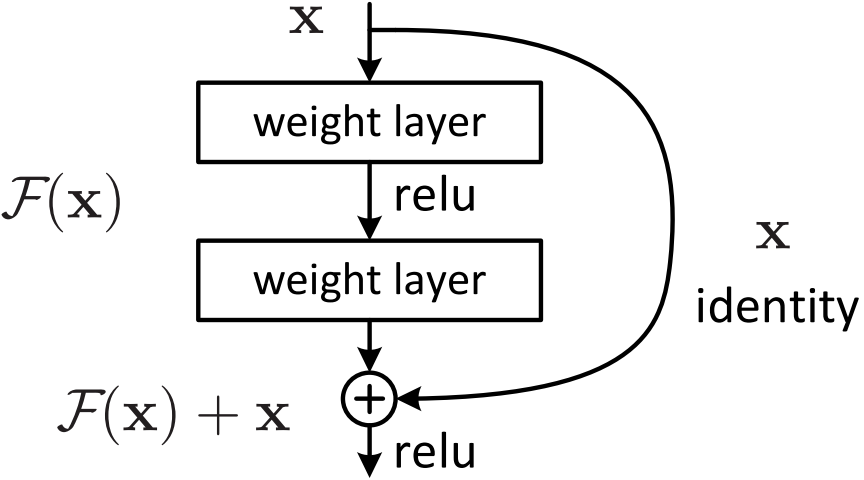
\includegraphics[width=0.5\linewidth]{img/resnet_building_block}
	\caption[Beispielhafter Baustein des ResNet]{Beispielhafter Baustein des ResNet~\cite{He.2016}}
	\label{fig:resnetbuildingblock}
\end{figure}

Bei der Objektdetektion und -lokalisierung in Bildern stellen die Autoren bei den ResNets deutliche Verbesserungen bei Steigerung der Netzfiefe fest im Gegensatz zu Referenzarchitekturen, bei denen eine Erhöhung der Tiefe eher noch eine Verschlechterung des Trainingsfehlers herbeiführt.
Erste Plätze bei Detektions- und Lokalisierungs-Challenges auf den Datasets ImageNet und COCO belegen die Wirksamkeit dieses Rest-Lernens.
Diesen Aufbau statt das U-Net als Grundlage für den Generator zu nehmen, könnte weitere Verbesserungen bei der Stabilisierung des Trainings bewirken.

Wie ein Segmentierungsnetz aussehen kann, das auf Rest-Lernen basiert, zeigen die \emph{RedNets} von \citeauthor{Mao.2016}~\cite{Mao.2016}.
Sehr gute Ergebnisse werden erzielt, wenn als Baustein zwei Ebenen aus Faltung, Rest-Lernen und Entfaltung gelernt werden (s.~\autoref{fig:rednetbuildingblock}).
Eine solche Architektur im Generator der \glspl{can} zu verwenden, könnte nicht nur zu besseren Ergebnissen, sondern auch zu besserer Stabilität im Training führen.

\begin{figure}
	\centering
	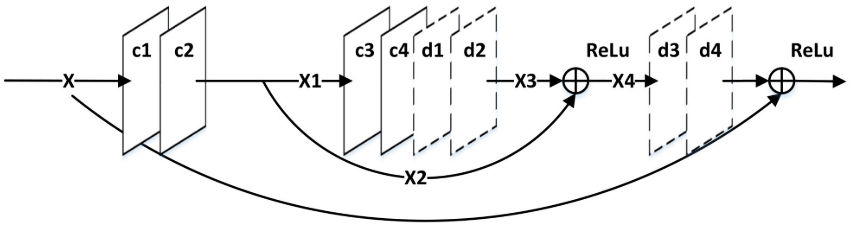
\includegraphics[width=0.8\linewidth]{img/rednet_building_block}
	\caption[Ein Baustein des RedNet]{Ein Baustein des RedNet~\cite{Mao.2016}. Kurven stehen für Skip Connections mit Identitätsmapping, voll umrandete Rechtecke für Faltungen (\emph{c1} etc.), gestrichelt umrandete für Entfaltungen (\emph{d1} etc.).}
	\label{fig:rednetbuildingblock}
\end{figure}



\section{Weiterentwicklungen der CANs}

Die Autoren der \glspl{can} haben ihren Ansatz bereits weiterentwickelt für eine Bild-zu-Bild-Übersetzung, bei der keine direkten Bild-zu-Bild-Paare zum Training zur Verfügung stehen~\cite{Zhu.2018}.
Stattdessen stehen eine \emph{Menge $ X $ an Inputs} einer \emph{Menge $ Y $ an Targets} gegenüber.
Mithilfe des GAN-Frameworks wird eine Projektion von $ X $ nach $ Y $ gelernt.
Diese wird mithilfe der Verlustfunktion auf Zyklenkonsistenz beschränkt, sodass nach einem Mapping von $ X $ nach $ Y $ das Mapping des Ergebnisses $ Y' $ auf $ X $ wieder ähnlich wie $ X $ sein muss.
Indem sie das GAN-Training mit einem Zyklenkonsistenz-Loss für beide Prädiktionsrichtungen kombinieren, übertreffen sie aktuelle Ansätze.
Für eine Multiklassen-Segmentierung verschlechtert sich allerdings das Ergebnis gegenüber den \glspl{can}.

\chapter{Fazit}

Die Segmentierung von Kolorektalpolypen in koloskopischem Bildmaterial kann Ärzte bei der Entdeckung von potenziell bösartigen Adenokarzinomen unterstützen.
\acrlongpl{can} sind eine Weiterentwicklung der \glspl{gan} und werden für eine Bild-zu-Bild-Übersetzung trainiert.

In dieser Masterarbeit wurden sie zum ersten Mal für eine Polypensegmentierung im Speziellen und für eine binäre Segmentierung generell verwendet.
% TODO Platz in GIANA Kategorie eintragen
Beim Training auf einem niedrigauflösenden Dataset der \gls{giana} Sub-Challenge 2018 erzielt das Netz einen durchschnittlichen \gls{iou} von 0,3681 auf den Testdaten und erreicht damit in der Kategorie "Polypen-Segmentierung SD" den [x.] Platz von [y].

Die visuelle Qualität der Segmentierungen ist nicht optimal, da sie oft kleine False Positives enthält.
Viele Erkenntnisse deuten darauf hin, dass die Zielrepräsentation, die das Netz lernen soll, reichhaltiger als ein spärliches Binärbild sein müsste.
Dennoch ist das \gls{can} in der Lage, eine binäre Segmentierung zu lernen.
Zukünftige Verbesserungen können in einer Stabilisierung des Trainings durch neue Verlustfunktionen und Generator-Architekturen liegen.


\listoffigures
\listoftables
\printglossary[type=\acronymtype,title={Abkürzungsverzeichnis}]
\printbibliography[heading=bibintoc]

\appendix
\chapter{Kurzdokumentation für die GIANA Sub-Challenge}
\includepdf[pages=-,fitpaper]{giana-doc/giana-polypsegsd-reutlingen.pdf}

%\clearpage
\addcontentsline{toc}{chapter}{Eidesstattliche Erklärung}
\chapter*{Eidesstattliche Erklärung}

Ich versichere, dass ich diese Arbeit selbstständig verfasst, keine anderen als die angegebenen Quellen und Hilfsmittel benutzt sowie alle wörtlich oder sinngemäß übernommenen Stellen in der Arbeit gekennzeichnet habe.
Die Arbeit wurde noch keiner Kommission zur Prüfung vorgelegt und verletzt in keiner Weise Rechte Dritter.

\begin{multicols}{2}
\underline{\hspace{5cm}}

(Ort, Datum)

\underline{\hspace{5cm}}

(Unterschrift)
\end{multicols}


\end{document}
